% !TEX root = ../main.tex
% ==============================================================================
% BAB 3: PEMODELAN DAN PERANCANGAN
% ==============================================================================

\chapter{PEMODELAN DAN PERANCANGAN}
\label{chapter:pemodelan-dan-perancangan}

Bab ini menguraikan secara komprehensif tahapan pemodelan dan perancangan platform \textit{Food AI Rescue} (FAR). Pembahasan difokuskan pada rancang bangun arsitektur sistem yang mengintegrasikan teknologi \textit{Progressive Web App} (PWA) dengan antarmuka Kecerdasan Buatan (AI). Selain itu, bab ini juga memetakan desain logika sistem dan struktur basis data relasional, perancangan antarmuka pengguna berbasis \textit{Human-Centered Design}, serta merincikan spesifikasi infrastruktur teknologi yang dibutuhkan untuk mendukung fase pengembangan hingga implementasi produksi platform.

% ==============================================================================
\section{Arsitektur Sistem}
% ==============================================================================

Arsitektur sistem merupakan gambaran menyeluruh mengenai bagaimana komponen perangkat lunak (\textit{software}) dan perangkat keras (\textit{hardware}) saling terhubung untuk menjalankan fungsi sistem secara efektif. Untuk memvisualisasikan hubungan tersebut, digunakan \textit{Deployment Diagram}, yaitu diagram yang merepresentasikan model fisik dari \textit{hardware} serta integrasi dan distribusi \textit{software} pada arsitektur perangkat keras tersebut.

Pada sistem Food AI Rescue, arsitektur dirancang menggunakan pendekatan \textit{client-server} terpisah, di mana berbagai segmen pengguna (donatur, penerima, relawan, admin, maupun \textit{super admin}) berinteraksi melalui \textit{web browser} (sebagai \textit{Client Frontend} berbasis React.ts) pada perangkat mereka. Seluruh permintaan (\textit{HTTP Request}) dari pengguna kemudian dikirimkan menuju \textit{Web Server} yang menjalankan lingkungan Node.js dan \textit{framework} Express sebagai \textit{backend}.

Dalam arsitektur ini, \textit{Web Server} bertugas sebagai pusat kendali untuk:
\begin{enumerate}
    \item Memproses berbagai permintaan dan interaksi dari pengguna.
    \item Mengelola autentikasi dan otorisasi akses (\textit{login/registrasi} berlapis).
    \item Menampilkan konten secara \textit{real-time}, seperti katalog ketersediaan surplus makanan, \textit{radar/map} penyaluran, dan Dasbor Dampak Sosial (SROI).
    \item Mengatur perhitungan algoritma gamifikasi berbasis poin (XP) dan \textit{leaderboard} bagi armada relawan.
    \item Mengintegrasikan layanan pihak ketiga (\textit{External Cloud Service}), yaitu dengan meneruskan permintaan gambar dan teks (\textit{API Request}) menuju server \textbf{Google Gemini AI} untuk proses verifikasi kelayakan makanan (``Polisi Pangan'') dan fitur \textit{AI Generatif}.
\end{enumerate}

Selain itu, \textit{Web Server} juga berkomunikasi secara eksklusif dengan \textit{Database Server} (MySQL) untuk melakukan pemrosesan, penyimpanan, dan pengambilan data, yang meliputi:
\begin{itemize}
    \item Data profil dan kredensial akun pengguna,
    \item Daftar inventaris surplus makanan beserta riwayat klaim/serah terima,
    \item Transaksi perolehan poin XP dan lencana (\textit{badge}) relawan,
    \item Rekapitulasi metrik keselamatan lingkungan (reduksi jejak karbon dan air).
\end{itemize}

Komunikasi antara \textit{Web Server} dan \textit{Database Server} dilakukan menggunakan \textit{SQL Query} (\textit{database request}) yang akan dibalas dengan \textit{SQL Result}. Seluruh lalu lintas data ini dipusatkan di \textit{Web Server} guna mencegah akses langsung klien ke \textit{database} maupun \textit{API Key}, sehingga keamanan sistem tetap terjaga.

Struktur teknis dari arsitektur sistem ini divisualisasikan pada Gambar \ref{fig:deployment-diagram} berikut dalam bentuk \textit{Deployment Diagram}, yang menunjukkan \textit{node} perangkat keras, layanan \textit{cloud}, serta relasi antarartefak perangkat lunak yang berjalan di dalamnya. Diagram ini berfungsi sebagai panduan penting dalam memahami implementasi fisik dan aliran data sistem Food AI Rescue saat dijalankan di lingkungan produksi.

% Placeholder: tambahkan gambar deployment diagram di sini
\begin{figure}[H]
    \centering
    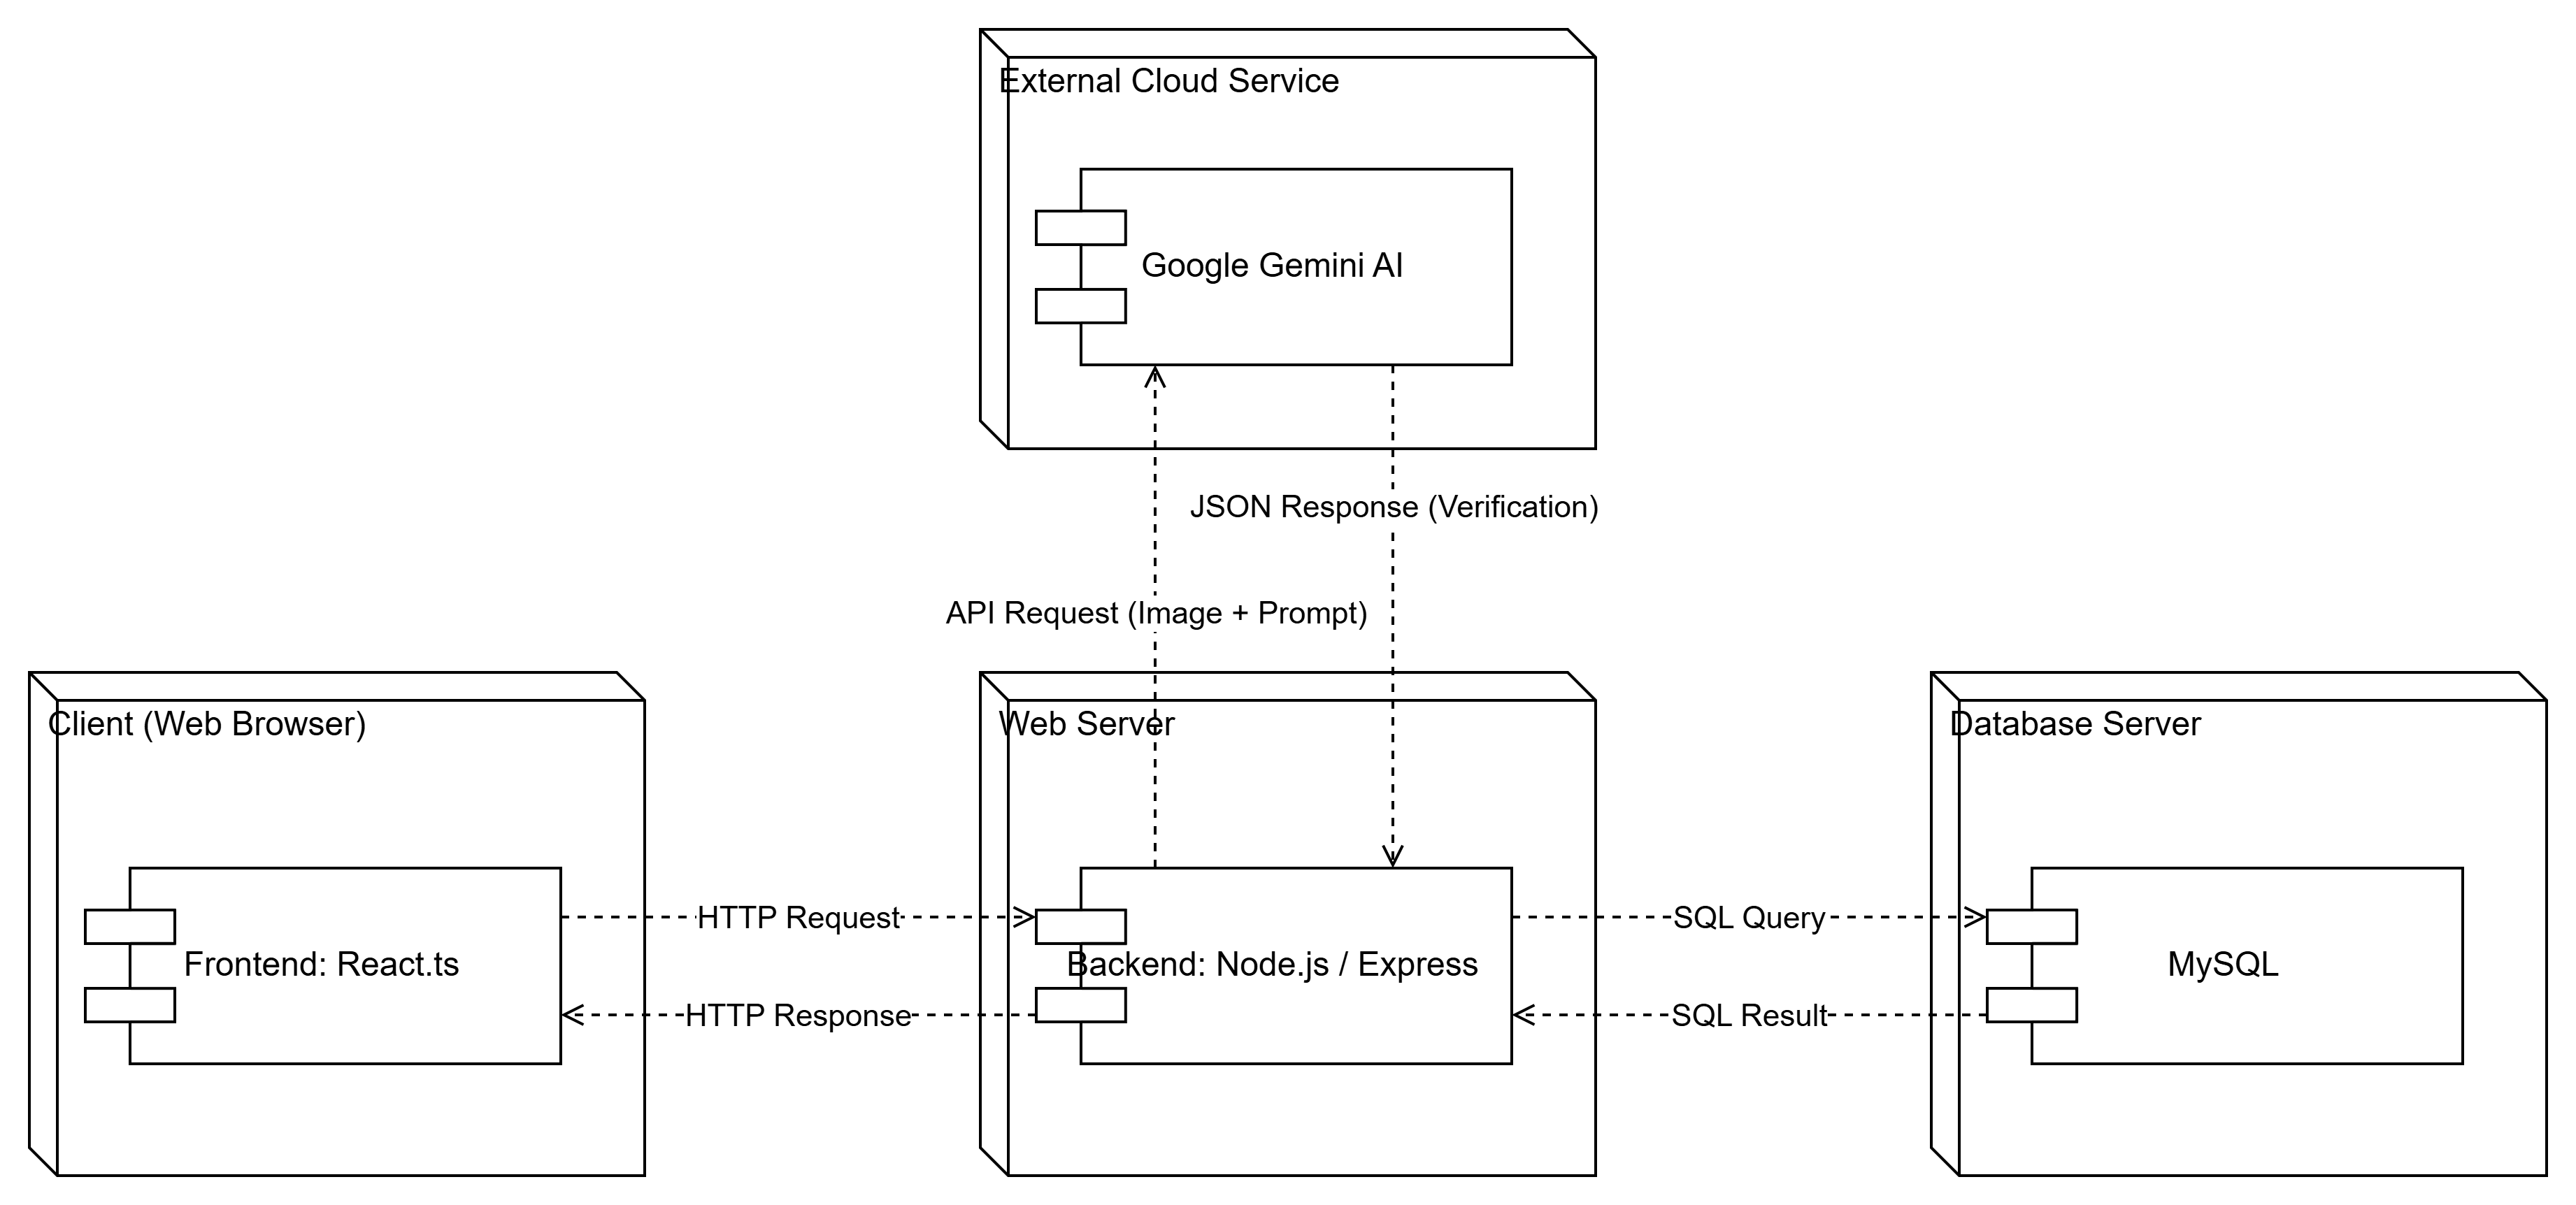
\includegraphics[width=1\textwidth]{image/bab3/Deployment Diagram Food AI Rescue.png}
    \caption{\textit{Deployment Diagram} Arsitektur Sistem Food AI Rescue}
    \label{fig:deployment-diagram}
\end{figure}

% ==============================================================================
\section{Pemodelan Sistem dan Data}
% ==============================================================================

Tahapan pemodelan sistem dan data bertujuan untuk memvisualisasikan alur interaksi aktor, struktur logika bisnis, dan organisasi penyimpanan informasi di dalam platform \textit{Food AI Rescue}. Rancang bangun ini direpresentasikan melalui serangkaian diagram analitis standar \textit{Unified Modeling Language} (UML) dan pemodelan relasional, yang meliputi \textit{Use Case Diagram} untuk memetakan batasan fungsional aktor, \textit{Entity Relationship Diagram} (ERD) untuk arsitektur pangkalan data, \textit{Class Diagram} untuk memetakan struktur objek pada peladen (\textit{server}), serta \textit{Sequence Diagram} untuk memvisualisasikan skenario pertukaran pesan dinamis pada fitur-fitur krusial.

% \subsection{\textit{Use Case Diagram}}
% \textit{Use Case Diagram} menggambarkan interaksi antara setiap aktor dengan fungsionalitas utama sistem Food AI Rescue. Terdapat 6 aktor utama yang berinteraksi dengan sistem, yaitu Donatur Individu, Donatur Korporat, Penerima, Relawan, Admin Pengelola, dan Super Admin.
%
% \begin{table}[H]
%     \centering
%     \caption{Deskripsi \textit{Use Case} Utama}
%     \label{tab:usecase}
%     \renewcommand{\arraystretch}{1.3}
%     \begin{tabular}{|p{2cm}|p{6cm}|p{6.5cm}|}
%         \hline
%         \textbf{Kode UC} & \textbf{Nama \textit{Use Case}} & \textbf{Aktor} \\
%         \hline
%         UC-01 & Unggah Donasi Makanan & Donatur Individu, Donatur Korporat \\
%         \hline
%         UC-02 & Verifikasi Kelayakan Makanan (AI) & Donatur Individu, Donatur Korporat \\
%         \hline
%         UC-03 & Klaim Donasi & Penerima \\
%         \hline
%         UC-04 & Pilih Metode Pengambilan & Penerima \\
%         \hline
%         UC-05 & Klaim Misi Pengantaran & Relawan \\
%         \hline
%         UC-06 & Pindai QR Code Serah Terima & Donatur, Relawan \\
%         \hline
%         UC-07 & Lihat Dasbor SROI & Donatur, Admin Pengelola \\
%         \hline
%         UC-08 & \textit{Generate} Konten AI Korporat & Donatur Korporat \\
%         \hline
%         UC-09 & Verifikasi Akun Pengguna & Admin Pengelola \\
%         \hline
%         UC-10 & Kelola \textit{Backend} Sistem & Super Admin \\
%         \hline
%     \end{tabular}
% \end{table}
%
% \noindent Berikut adalah narasi singkat untuk \textit{use case} inti sistem:
%
% \begin{description}
%     \item[UC-01 – Unggah Donasi Makanan:] Donatur mengunggah data makanan surplus meliputi foto, deskripsi, jumlah porsi, dan lokasi. Sebelum dipublikasikan, sistem mewajibkan donatur untuk menjalankan UC-02.
%     \item[UC-02 – Verifikasi Kelayakan Makanan (AI):] Donatur memindai foto makanan menggunakan kamera. Sistem mengirimkan gambar ke \textit{Google Gemini Vision API} untuk dianalisis kelayakan fisik, higienitas visual, dan kehalalannya. Hasil verifikasi ditampilkan secara instan.
%     \item[UC-06 – Pindai QR Code Serah Terima:] Merupakan \textit{use case} kritis untuk mencegah klaim ganda. Pada metode \textit{pick-up}, Donatur memindai QR Code Penerima. Pada metode diantar, Donatur memindai QR Code Relawan, kemudian Relawan memindai QR Code Penerima.
%     \item[UC-08 – Generate Konten AI Korporat:] Eksklusif untuk Donatur Korporat. Mencakup fitur \textit{Eco Packaging Editor} untuk menghasilkan desain kemasan ramah lingkungan dan \textit{CSR Copywriter} untuk menghasilkan konten promosi media sosial secara otomatis.
% \end{description}

\subsection{\textit{Use Case}}

\subsection{\textit{Entity Relationship Diagram} (ERD)}
ERD berikut menggambarkan struktur basis data relasional yang menjadi fondasi penyimpanan data platform Food AI Rescue. Entitas utama dan relasinya dijabarkan sebagai berikut:

\begin{longtable}{|p{4.5cm}|p{6cm}|p{4cm}|}
    \caption{Daftar Seluruh Entitas Basis Data Food AI Rescue}
    \label{tab:erd-entities-full} \\
    \hline
    \textbf{Entitas} & \textbf{Atribut Utama} & \textbf{Keterangan} \\
    \hline
    \endfirsthead
    \hline
    \textbf{Entitas} & \textbf{Atribut Utama} & \textbf{Keterangan} \\
    \hline
    \endhead
    \hline
    \multicolumn{3}{r}{\textit{Bersambung ke halaman berikutnya}} \\
    \endfoot
    \hline
    \endlastfoot
    \tbltt{addresses} & id, user\_id, label, full\_address, latitude, longitude, is\_primary & Titik lokasi dan alamat pengguna \\
    \hline
    \tbltt{admin\_targets} & id, metric\_key, target\_value, label & Konfigurasi target metrik admin \\
    \hline
    \tbltt{ai\_verifications} & id, food\_id, is\_edible, halal\_score, quality\_score, reason, allergens & Log hasil verifikasi kelayakan oleh AI \\
    \hline
    \tbltt{badges} & id, name, role, min\_points, icon, description & Sistem lencana untuk gamifikasi \\
    \hline
    \tbltt{broadcasts} & id, title, content, target, type, author\_id & Pengumuman atau siaran sistem \\
    \hline
    \tbltt{broadcast\_reads} & user\_id, broadcast\_id, read\_at & Status keterbacaan pengumuman \\
    \hline
    \tbltt{claims} & id, food\_id, receiver\_id, volunteer\_id, claimed\_quantity, status & Data transaksi klaim dan pengantaran \\
    \hline
    \tbltt{corporate\_ai\_generations} & id, donor\_id, food\_id, type, title, content & Data hasil AI generatif untuk korporat \\
    \hline
    \tbltt{email\_verifications} & id, email, code, expires\_at & Data kode verifikasi email \\
    \hline
    \tbltt{faqs} & id, category, question, answer & Pertanyaan yang sering diajukan \\
    \hline
    \tbltt{food\_items} & id, provider\_id, name, current\_quantity, category, status & Data pasokan dan donasi makanan \\
    \hline
    \tbltt{food\_requests} & id, receiver\_id, title, description, needed\_quantity, status & Permintaan spesifik donasi makanan \\
    \hline
    \tbltt{leaderboard\_snapshots} & id, user\_id, points, rank, period, snapshot\_date & Rekaman riwayat peringkat pengguna \\
    \hline
    \tbltt{notifications} & id, user\_id, type, title, message, is\_read & Sistem notifikasi pengguna \\
    \hline
    \tbltt{password\_resets} & id, user\_id, token, expires\_at & Token untuk pemulihan kata sandi \\
    \hline
    \tbltt{point\_histories} & id, user\_id, amount, activity\_type, reference\_id & Riwayat perolehan poin gamifikasi \\
    \hline
    \tbltt{quests} & id, title, description, target\_value, reward\_points & Daftar misi harian/spesifik gamifikasi \\
    \hline
    \tbltt{rank\_levels} & id, role, name, min\_points, benefits, color & Tingkatan level (pangkat) pengguna \\
    \hline
    \tbltt{reports} & id, reporter\_id, claim\_id, category, status, is\_urgent & Laporan aduan atau kendala donasi \\
    \hline
    \tbltt{reviews} & id, claim\_id, user\_id, partner\_id, food\_id, rating & Ulasan dan penilaian pasca-donasi \\
    \hline
    \tbltt{social\_impacts} & id, food\_id, co2\_per\_portion, water\_saved\_liter, land\_saved\_sqm & Metrik kalkulasi dampak sosial lingkungan \\
    \hline
    \tbltt{system\_logs} & id, actor\_id, actor\_name, action, severity & Catatan aktivitas di dalam sistem \\
    \hline
    \tbltt{system\_settings} & setting\_key, setting\_value, updated\_at & Pengaturan dinamis platform \\
    \hline
    \tbltt{users} & id, name, email, password, role, status, points, avatar & Data profil utama seluruh pengguna \\
    \hline
    \tbltt{user\_ai\_keys} & id, user\_id, api\_key, label & Kunci API pribadi milik pengguna \\
    \hline
    \tbltt{user\_impact\_stats} & user\_id, total\_waste\_kg, total\_co2\_kg, total\_water\_liter & Akumulasi total dampak tiap pengguna \\
    \hline
    \tbltt{user\_quests} & id, user\_id, quest\_id, current\_value, is\_completed & Progres pengerjaan misi pengguna \\
    \hline
    \tbltt{verification\_codes} & id, identifier, channel, email, code, type, expires\_at & Kode OTP multi-saluran \\
    \hline
\end{longtable}

\newpage
\begin{landscape}
    \centering
    \vfill
    \includegraphics[width=\linewidth, height=0.85\textheight, keepaspectratio]{image/bab3/erd.png}
    \captionsetup{hypcap=false}
    \captionof{figure}{Entity Relationship Diagram (ERD) Food AI Rescue}
    \label{fig:erd}
    \vfill
\end{landscape}

\newpage

\noindent Relasi antar entitas utama adalah sebagai berikut:
\begin{itemize}
    \item Satu \texttt{users} (donatur) dapat memiliki banyak \texttt{donations} (relasi \textit{one-to-many}).
    \item Satu \texttt{donations} dapat memiliki banyak \texttt{claims}, namun hanya satu klaim yang berstatus aktif pada satu waktu untuk mencegah \textit{double-claim}.
    \item Satu \texttt{claims} memiliki tepat satu \texttt{deliveries} jika metode pengantaran yang dipilih adalah ``Diantar Relawan''.
    \item Setiap \texttt{donations} yang berhasil diselesaikan akan menghasilkan satu entri pada \texttt{sroi\_records}.
    \item Setiap \texttt{users} (relawan) memiliki satu entri pada \texttt{leaderboard} yang diperbarui setiap misi selesai.
\end{itemize}

\subsection{\textit{Class Diagram}}
\textit{Class Diagram} (Diagram Kelas) pada aplikasi \textit{Food AI Rescue} (FAR) dimodelkan menggunakan pendekatan \textit{Service-Oriented Architecture} (SOA) yang memisahkan antara entitas data (Model), layanan pemroses (\textit{Service}/\textit{Utility}), dan antarmuka pengguna (\textit{Component}). Pemisahan ini ditandai dengan penggunaan \textit{stereotype} (seperti \texttt{<<entity>>}, \texttt{<<service>>}, dan \texttt{<<component>>}) guna mengidentifikasi peran masing-masing kelas di dalam sistem.

Rincian spesifikasi kelas, deskripsi fungsi, beserta daftar atribut dan metode (operasi) yang menyertainya dijabarkan secara lengkap pada Tabel \ref{tab:class-diagram} berikut:

\begin{longtable}{|p{0.4cm}|p{2.8cm}|p{3.5cm}|p{3cm}|p{3.8cm}|}
    \caption{Spesifikasi dan Penjelasan \textit{Class Diagram}}
    \label{tab:class-diagram} \\
    \hline
    \textbf{No} & \textbf{Nama Kelas \& \textit{Stereotype}} & \textbf{Deskripsi / Fungsi} & \textbf{Atribut Utama} & \textbf{Operasi / Metode Utama} \\
    \hline
    \endfirsthead
    \hline
    \textbf{No} & \textbf{Nama Kelas \& \textit{Stereotype}} & \textbf{Deskripsi / Fungsi} & \textbf{Atribut Utama} & \textbf{Operasi / Metode Utama} \\
    \hline
    \endhead
    \hline
    \multicolumn{5}{r}{\textit{Bersambung ke halaman berikutnya}} \\
    \endfoot
    \hline
    \endlastfoot

    1 & \textbf{System Enums} \newline \texttt{<<enumeration>>} & Kumpulan tipe data statis konstan yang digunakan untuk membatasi nilai input (seperti jenis peran, status makanan, dan metode pengiriman) guna mencegah anomali data di seluruh sistem. & \tbltt{UserRole, FoodStatus, ClaimStatus, DeliveryMethod} & \textit{(Tidak memiliki operasi/metode, hanya berisi nilai konstan)} \\
    \hline

    2 & \textbf{UserData} \newline \texttt{<<entity>>} & Merepresentasikan model data profil pengguna terdaftar, termasuk penyimpanan kredensial, peran (\textit{role}), dan total poin kontribusi (SROI/XP). & \tbltt{id, name, email, role, status, points, phone, address, password} & \tbltt{authenticate(), updatePoints(), verifyOTP()} \\
    \hline

    3 & \textbf{FoodItem} \newline \texttt{<<entity>>} & Merepresentasikan model data inventaris makanan surplus dari donatur. Menyimpan data kuantitas, waktu kadaluarsa, hingga hasil JSON verifikasi AI dan kalkulasi dampak sosial. & \tbltt{id, providerId, name, currentQuantity, expiryTime, aiVerification, socialImpact} & \tbltt{deductStock(), checkExpiry(), updateStatus()} \\
    \hline

    4 & \textbf{ClaimHistoryItem} \newline \texttt{<<entity>>} & Merepresentasikan model log transaksi pesanan yang menghubungkan entitas Donatur, Penerima, dan Relawan. Menyimpan kode unik serah terima dan data ulasan. & \tbltt{id, foodId, receiverId, volunteerId, uniqueCode, status, rating, review} & \tbltt{generateQR(), assignVolunteer(), scanAndComplete()} \\
    \hline

    5 & \textbf{Address} \newline \texttt{<<entity>>} & Model data yang menyimpan detail koordinat geolokasi dan alamat fisik pengguna untuk keperluan pemetaan dan penjemputan logistik. & \tbltt{id, userId, label, fullAddress, lat, lng, contactPhone} & \textit{(Sebagai entitas data murni, dimanipulasi oleh layanan basis data)} \\
    \hline

    6 & \textbf{DatabaseService} \newline \texttt{<<service>>} & Modul \textit{backend} utama yang bertugas mengelola koneksi dan mengeksekusi kueri langsung ke basis data MySQL (proses CRUD transaksi). & \tbltt{API\_URL, headers} & \tbltt{registerUser(), loginUser(), addFoodItem(), processClaimTransaction(), getClaims()} \\
    \hline

    7 & \textbf{AIService} \newline \texttt{<<service>>} & Layanan integrasi sistem cerdas yang menangani komunikasi (API \textit{Call}) ke model \textit{Google Gemini} untuk validasi makanan dan \textit{Generate} CSR. & \tbltt{apiKeys, currentKeyIndex, model} & \tbltt{verifyFoodSafety(), generateCSRContent(), designPackaging(), rotateKey()} \\
    \hline

    8 & \textbf{FileService} \newline \texttt{<<service>>} & Modul pengelola media untuk menangani kompresi, penyimpanan (\textit{upload}), dan penghapusan berkas gambar/foto ke dalam direktori lokal server. & \tbltt{uploadPath, maxFileSize} & \tbltt{uploadImage(), optimizeImage(), deleteFile()} \\
    \hline

    9 & \textbf{GamificationService} \newline \texttt{<<utility>>} & Skrip utilitas (\textit{helper}) yang berisi logika kalkulasi untuk menghitung \textit{Experience Point} (XP), menentukan pangkat (\textit{rank}), dan memberikan lencana ke pengguna. & \tbltt{rankLevels, badges} & \tbltt{calculateXP(), evaluateRank(), awardBadge(), getLeaderboard()} \\
    \hline

    10 & \textbf{ExpiryChecker} \newline \texttt{<<utility>>} & Pekerja latar belakang (\textit{background job}) yang secara berkala memeriksa waktu dan mengubah status makanan jika telah melewati batas waktu aman konsumsi. & \textit{(Skrip berjalan independen tanpa atribut state tetap)} & \tbltt{checkAndExpireItems(), isFoodExpired()} \\
    \hline

    11 & \textbf{App} \newline \texttt{<<component>>} & Komponen akar (\textit{root}) dari \textit{Frontend} (React) yang bertindak sebagai \textit{router} utama pengelola sesi dan pengarah antarmuka ke dasbor masing-masing \textit{role}. & \tbltt{currentView, role, currentUser, isDarkMode} & \tbltt{handleLogin(), handleLogout(), handleClaimFood(), renderContent()} \\
    \hline

    12 & \textbf{ProviderIndex} \newline \texttt{<<component>>} & Komponen antarmuka pengguna untuk Donatur (Individu/Korporat). Mengelola UI inventaris, riwayat donasi, dan pemicu alat AI Korporat. & \tbltt{foodItems, claimHistory} & \tbltt{renderDashboard(), renderInventory(), renderOrders()} \\
    \hline

    13 & \textbf{ReceiverIndex} \newline \texttt{<<component>>} & Komponen antarmuka pengguna untuk Penerima. Mengelola UI katalog makanan yang tersedia dan formulir penyelesaian klaim/laporan. & \tbltt{availableFood, selectedFood} & \tbltt{renderFoodList(), renderFoodDetail(), handleClaim()} \\
    \hline

    14 & \textbf{VolunteerIndex} \newline \texttt{<<component>>} & Komponen antarmuka pengguna untuk Relawan. Mengelola UI papan misi (\textit{Missions Board}) geografis dan visualisasi \textit{leaderboard} gamifikasi. & \tbltt{missions, leaderboard} & \tbltt{renderMissions(), acceptMission(), renderLeaderboard()} \\
    \hline

    15 & \textbf{AdminIndex} \newline \texttt{<<component>>} & Komponen antarmuka pengguna panel kontrol untuk Administrator. Digunakan untuk memoderasi laporan sengketa dan memverifikasi pengguna baru. & \tbltt{users, reports, systemLogs} & \tbltt{renderCommunity(), renderModeration(), verifyUser()} \\
    \hline

\end{longtable}

\noindent Hubungan antar kelas yang penting:
\begin{itemize}
    \item \texttt{App} (\texttt{<<component>>}) bertindak sebagai orkestrator utama yang menginstansiasi \texttt{DatabaseService} dan \texttt{AIService} untuk seluruh operasi data dan AI.
    \item \texttt{FoodItem} berasosiasi dengan \texttt{AIService} melalui atribut \texttt{aiVerification} yang diisi setelah proses \texttt{verifyFoodSafety()} selesai.
    \item \texttt{ClaimHistoryItem} berasosiasi dengan \texttt{GamificationService} — setiap kali \texttt{scanAndComplete()} dipanggil, sistem memicu \texttt{calculateXP()} dan \texttt{evaluateRank()}.
    \item \texttt{ExpiryChecker} memantau seluruh entitas \texttt{FoodItem} secara periodik dan memanggil \texttt{updateStatus()} jika makanan telah melewati \texttt{expiryTime}.
    \item \texttt{FileService} digunakan oleh \texttt{DatabaseService} setiap kali ada operasi unggah foto makanan atau aset AI generatif.
\end{itemize}

\newpage
\begin{landscape}
    \centering
    \vfill
    \includesvg[width=\linewidth, height=0.85\textheight, keepaspectratio, inkscapelatex=false]{image/bab3/class diagram}
    \captionsetup{hypcap=false}
    \captionof{figure}{\textit{Class Diagram} Food AI Rescue}
    \label{fig:class-diagram}
    \vfill
\end{landscape}
\newpage

\subsection{\textit{Sequence Diagram}}
\textit{Sequence diagram} merupakan grafik dua dimensi di mana objek ditunjukkan pada dimensi horizontal, sedangkan garis waktu (\textit{lifeline}) ditunjukkan pada dimensi vertikal. Pada sistem Food AI Rescue, \textit{Sequence Diagram} digunakan untuk memvisualisasikan urutan interaksi antara pengguna (aktor) dan berbagai komponen sistem dalam mengeksekusi sebuah proses. Diagram ini menguraikan secara terperinci bagaimana aliran pesan (\textit{message}) dikirim dan diterima secara berurutan, dimulai dari interaksi pengguna pada antarmuka aplikasi (\textit{Client/Frontend}), pemrosesan permintaan oleh peladen (\textit{Backend API}), integrasi dengan layanan Kecerdasan Buatan (\textit{Google Gemini AI}), hingga proses penyimpanan dan pemberian respons oleh basis data (\textit{Database}).

Untuk memberikan gambaran teknis yang lebih komprehensif, berikut ini disajikan rincian \textit{sequence diagram} yang memetakan seluruh alur proses utama pada sistem Food AI Rescue.

% ------------------------------------------------------------------
\subsubsection{Alur Global (Umum)}
% ------------------------------------------------------------------

\textbf{1. \textit{Sequence Diagram} Melakukan \textit{Login} (Global)}

Pengguna memasukkan email dan kata sandi di Halaman \textit{Login}. Sistem mengirimkan perintah \texttt{validateLogin(email, password)} ke \textit{Auth Service}. Layanan ini kemudian melakukan kueri ke \textit{Database} untuk memverifikasi kredensial. Jika kredensial salah, \textit{Database} menyatakan data tidak ditemukan dan pesan \textit{error} ditampilkan ke pengguna. Jika benar, sistem melakukan \textit{Generate JWT Token \& Session}, mengirimkan token kesuksesan, dan me-\textit{redirect} pengguna ke \textit{Dashboard Role} masing-masing secara spesifik.

\begin{figure}[H]
    \centering
    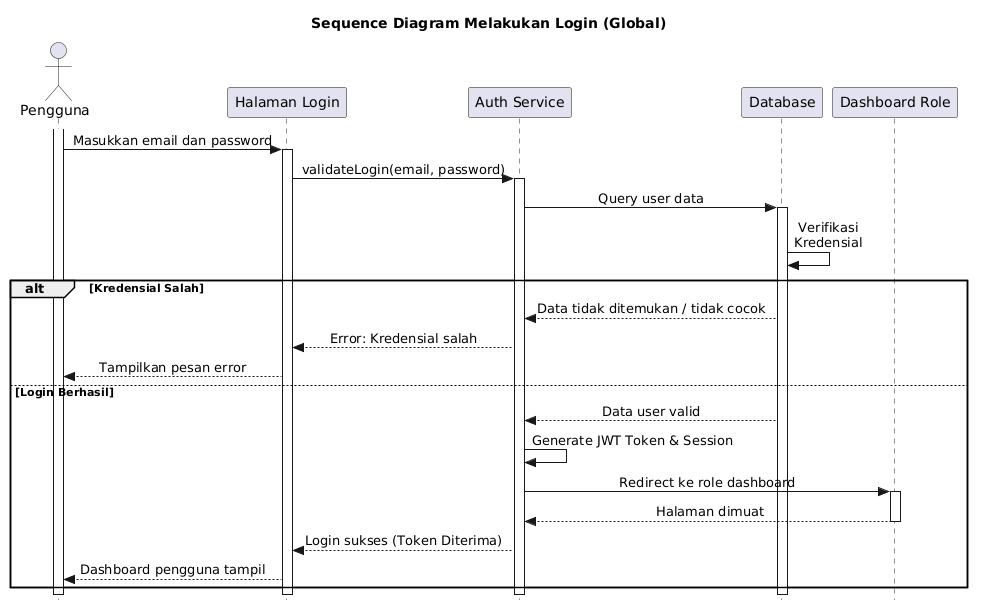
\includegraphics[width=1\textwidth]{image/bab3/sequence/Sequence Diagram Melakukan Login (Global).png}
    \captionsetup{hypcap=false}
    \caption{\textit{Sequence Diagram} Melakukan \textit{Login} (Global)}
    \label{fig:sd-login}
\end{figure}

% ------------------------------------------------------------------
\subsubsection{Alur Donatur (Individu \& Korporat)}
% ------------------------------------------------------------------

\textbf{2. \textit{Sequence Diagram} Unggah Surplus Makanan \& Verifikasi AI}

Donatur mengisi data makanan dan mengunggah fotonya melalui \textit{Form Upload}. Sistem mengirim data tersebut (\texttt{verifyFoodData}) ke \textit{Backend API}. \textit{Backend} kemudian mengirimkan instruksi teks (\textit{prompt}) beserta foto ke layanan \textbf{Google Gemini API}. Gemini merespons dengan JSON berisi skor keamanan, daftar bahan, alergen, dan skor sosial. Hasil ini ditampilkan ke donatur. Jika donatur menekan ``Publikasikan'', fungsi \texttt{publishFoodItem} dipanggil, data disimpan ke \textit{Database}, dan status makanan berubah menjadi \textit{AVAILABLE}.

\begin{figure}[H]
    \centering
    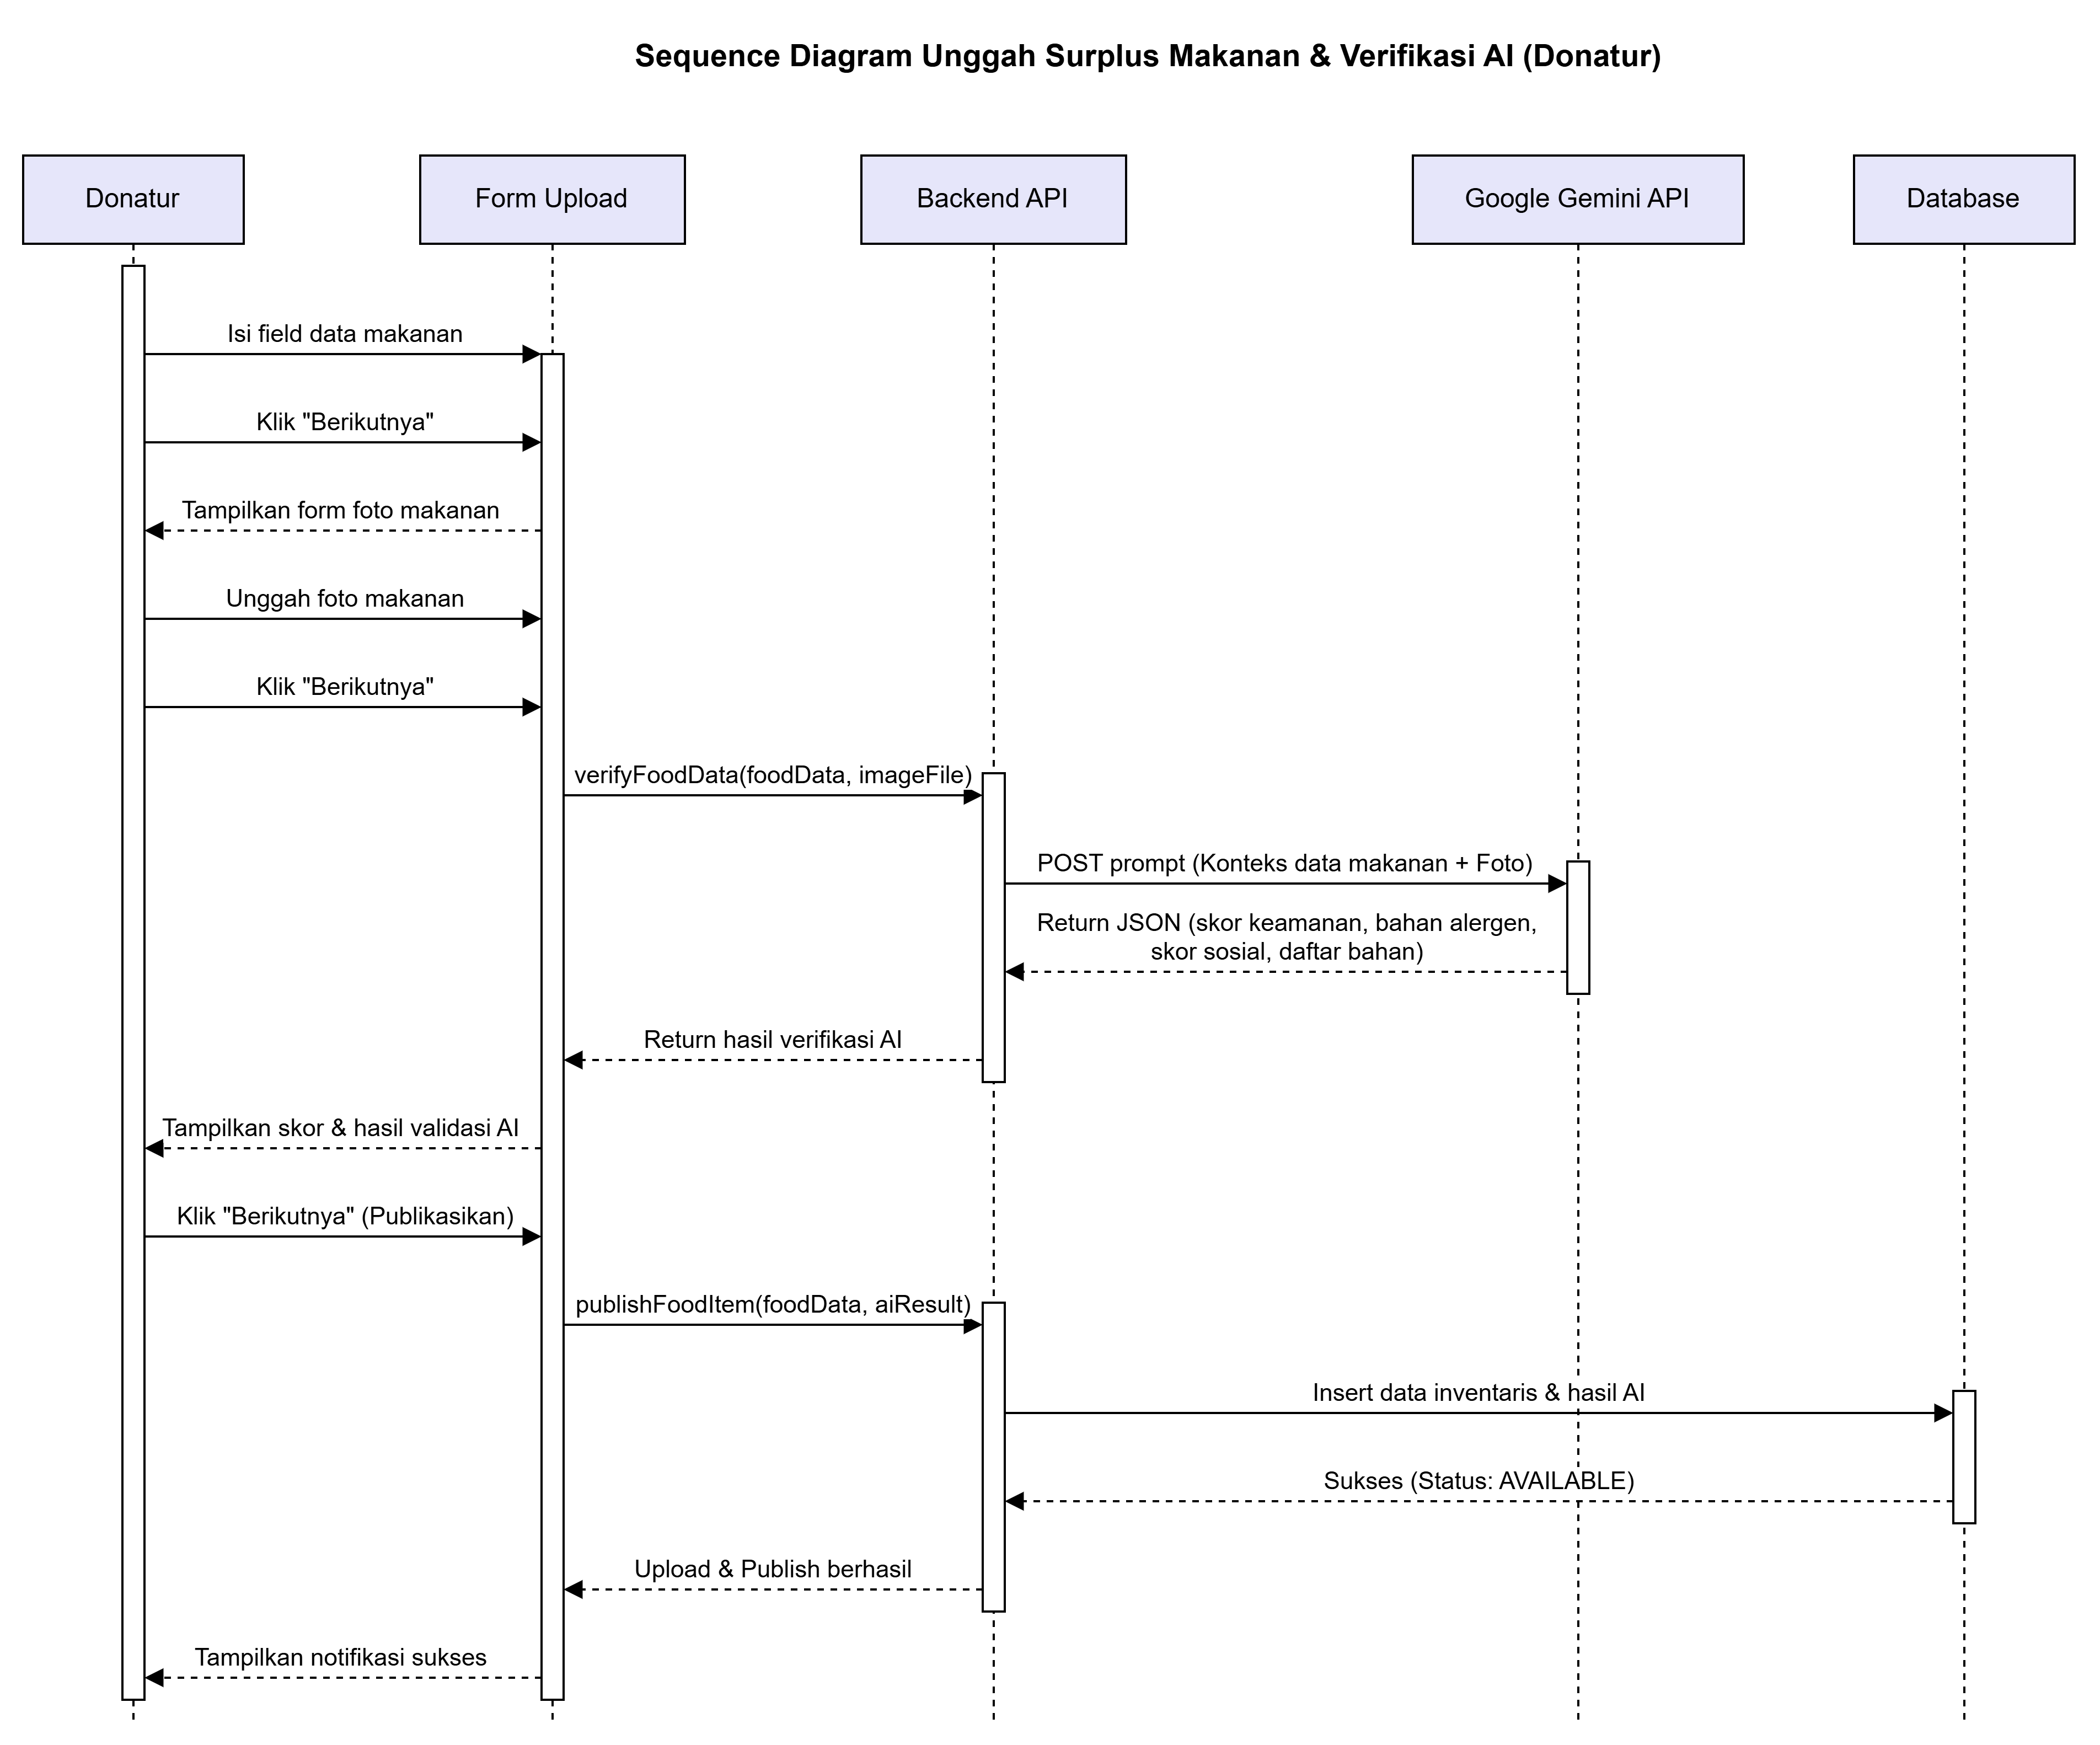
\includegraphics[width=1\textwidth]{image/bab3/sequence/Sequence Diagram Unggah Surplus Makanan & Verifikasi AI (Donatur).png}
    \captionsetup{hypcap=false}
    \caption{\textit{Sequence Diagram} Unggah Surplus Makanan \& Verifikasi AI (Donatur)}
    \label{fig:sd-upload-donatur}
\end{figure}

\textbf{3. \textit{Sequence Diagram} Konfirmasi Pesanan}

Donatur melihat daftar pesanan yang masuk dan mengklik ``Terima''. \textit{Dashboard} mengirim perintah \texttt{handleApproveClaim(claimId)} ke \textit{Backend}. \textit{Backend} memperbarui status klaim menjadi \textit{APPROVED/READY} di \textit{Database}, lalu mengirimkan notifikasi ke Penerima atau Relawan bahwa pesanan ``Siap Diambil''.

\begin{figure}[H]
    \centering
    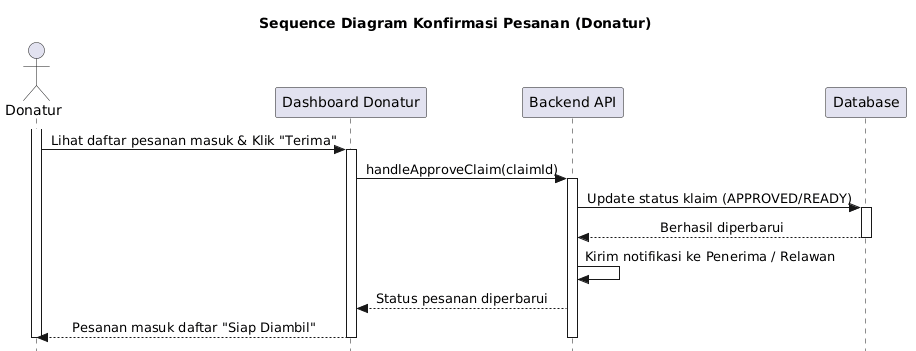
\includegraphics[width=1\textwidth]{image/bab3/sequence/Sequence Diagram Konfirmasi Pesanan (Donatur).png}
    \captionsetup{hypcap=false}
    \caption{\textit{Sequence Diagram} Konfirmasi Pesanan (Donatur)}
    \label{fig:sd-konfirmasi-donatur}
\end{figure}

\textbf{4. \textit{Sequence Diagram} Dasbor Dampak Sosial SROI \& Jejak Karbon}

Donatur membuka halaman Dampak Sosial. Antarmuka memanggil \texttt{fetchImpactStats(userId)} ke \textit{Backend}. \textit{Backend} melakukan agregasi kalkulasi pencegahan limbah (\texttt{waste\_kg}) dan karbon (\texttt{co2\_kg}) dari \textit{Database}. Hasil statistik dikembalikan dalam format JSON untuk dirender menjadi grafik CO\textsubscript{2} yang interaktif pada antarmuka pengguna.

\begin{figure}[H]
    \centering
    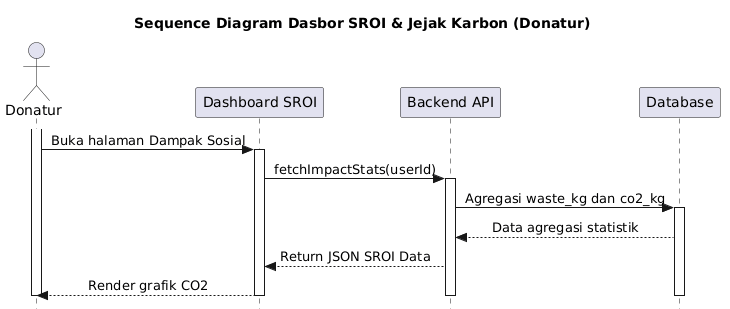
\includegraphics[width=1\textwidth]{image/bab3/sequence/Sequence Diagram Dasbor Dampak Sosial SROI (Donatur).png}
    \captionsetup{hypcap=false}
    \caption{\textit{Sequence Diagram} Dasbor Dampak Sosial SROI (Donatur)}
    \label{fig:sd-sroi-donatur}
\end{figure}

% ------------------------------------------------------------------
\subsubsection{Alur Eksklusif Donatur Korporat (AI Generatif)}
% ------------------------------------------------------------------

\textbf{5. \textit{Sequence Diagram} Pembuatan Logo \& Rekomendasi Kemasan}

Donatur Korporat memasukkan daftar makanan dan instruksi logo di \textit{Packaging Studio}. Studio memanggil \texttt{generatePackagingSolution} ke \textit{AI Service}. AI kemudian mengirim \textit{POST prompt image} ke Gemini API untuk membuat logo, dan \textit{POST prompt text} untuk mencari rekomendasi material ramah lingkungan. URL gambar dan teks rekomendasi dikembalikan untuk ditampilkan ke pengguna.

\begin{figure}[H]
    \centering
    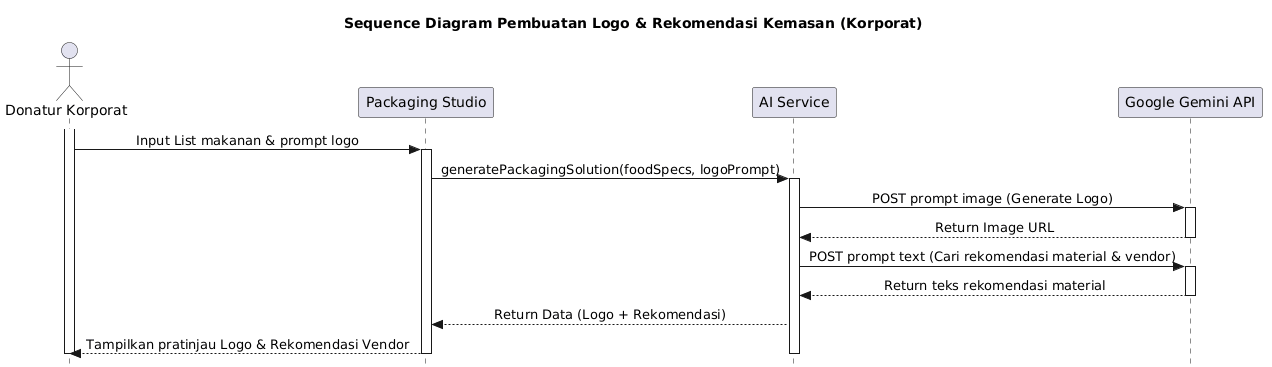
\includegraphics[width=1\textwidth]{image/bab3/sequence/Sequence Diagram Pembuatan Logo & Rekomendasi Kemasan (Korporat).png}
    \captionsetup{hypcap=false}
    \caption{\textit{Sequence Diagram} Pembuatan Logo \& Rekomendasi Kemasan (Donatur Korporat)}
    \label{fig:sd-kemasan-korporat}
\end{figure}

\textbf{6. \textit{Sequence Diagram} \textit{Generate} CSR \textit{Copywriter}}

Pengguna korporat memilih jenis makanan, nada bahasa (\textit{tone}), dan platform media sosial pada \textit{CSR Editor}. Sistem memanggil \textit{AI Service}, yang pertama-tama mengambil spesifikasi donasi dari \textit{Database}. AI kemudian mengirim instruksi ke Gemini API untuk membuat 2 versi takarir (\textit{caption}). Draf ini disimpan ke tabel \texttt{corporate\_ai\_generations} di \textit{database} sebelum ditampilkan ke pengguna.

\begin{figure}[H]
    \centering
    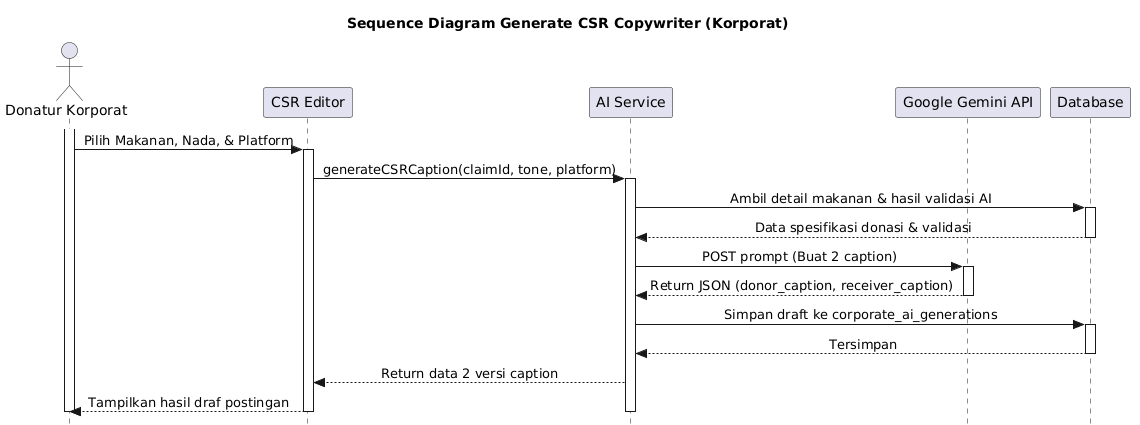
\includegraphics[width=1\textwidth]{image/bab3/sequence/Sequence Diagram Generate CSR Copywriter (Korporat).png}
    \captionsetup{hypcap=false}
    \caption{\textit{Sequence Diagram} \textit{Generate} CSR \textit{Copywriter} (Donatur Korporat)}
    \label{fig:sd-csr-korporat}
\end{figure}

% ------------------------------------------------------------------
\subsubsection{Alur Penerima Donasi}
% ------------------------------------------------------------------

\textbf{7. \textit{Sequence Diagram} Pencarian \& Klaim Makanan}

Penerima memilih makanan dan metode pengambilan, lalu mengklik ``Klaim''. \textit{Backend} menerima \texttt{handleClaimFood} dan mengecek ketersediaan stok di \textit{Database}. Jika stok habis, proses digagalkan. Jika tersedia, \textit{Backend} akan men-\textit{generate Unique Code} (Kode QR), melakukan kalkulasi dampak, mengurangi stok di \textit{database}, dan menyimpan klaim baru. Antarmuka kemudian menampilkan \textit{Success Splash Screen}.

\begin{figure}[H]
    \centering
    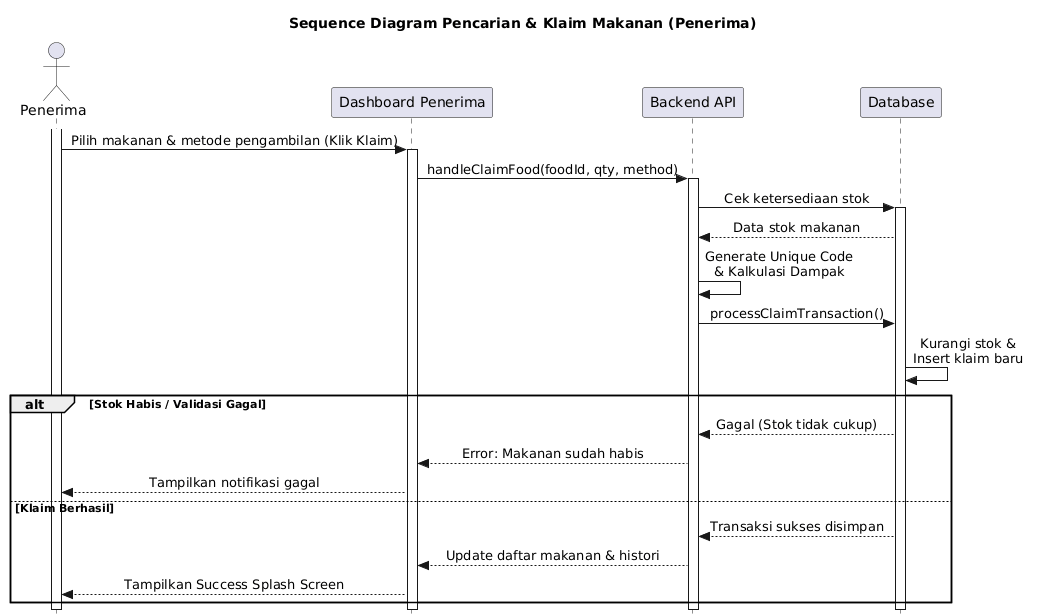
\includegraphics[width=1\textwidth]{image/bab3/sequence/Sequence Diagram Pencarian & Klaim Makanan (Penerima).png}
    \captionsetup{hypcap=false}
    \caption{\textit{Sequence Diagram} Pencarian \& Klaim Makanan (Penerima)}
    \label{fig:sd-klaim-penerima}
\end{figure}

\textbf{8. \textit{Sequence Diagram} Pelaporan Masalah}

Penerima mengisi alasan dan mengunggah bukti di \textit{Modal} Laporan (misal jika makanan rusak). \textit{Backend} memproses \texttt{handleSubmitReport}, menyimpan data ke \textit{Database} (memperbarui status klaim), dan memicu \texttt{insertAdminNotification()}. Jika sukses, lencana status klaim berubah menjadi ``Reported''.

\begin{figure}[H]
    \centering
    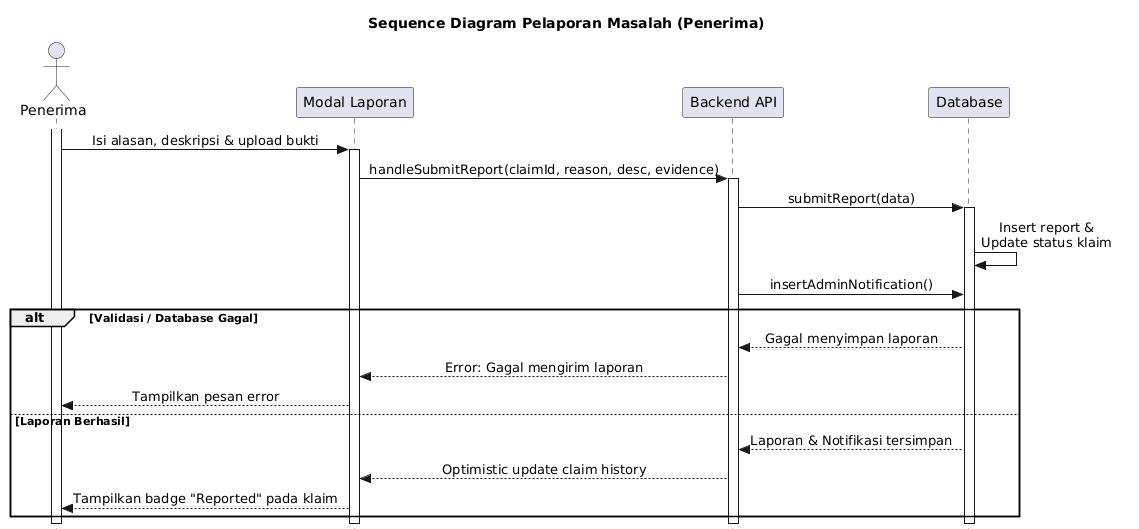
\includegraphics[width=1\textwidth]{image/bab3/sequence/Sequence Diagram Pelaporan Masalah (Penerima).png}
    \captionsetup{hypcap=false}
    \caption{\textit{Sequence Diagram} Pelaporan Masalah (Penerima)}
    \label{fig:sd-laporan-penerima}
\end{figure}

\textbf{9. \textit{Sequence Diagram} Pemberian Ulasan}

Setelah makanan diterima, Penerima mengisi \textit{rating} dan komentar. \textit{Backend} menerima \texttt{handleSubmitReview} dan menyimpannya ke \textit{Database}. Jika berhasil, kartu klaim pada riwayat pengguna akan diperbarui menjadi berstatus ``Reviewed''.

\begin{figure}[H]
    \centering
    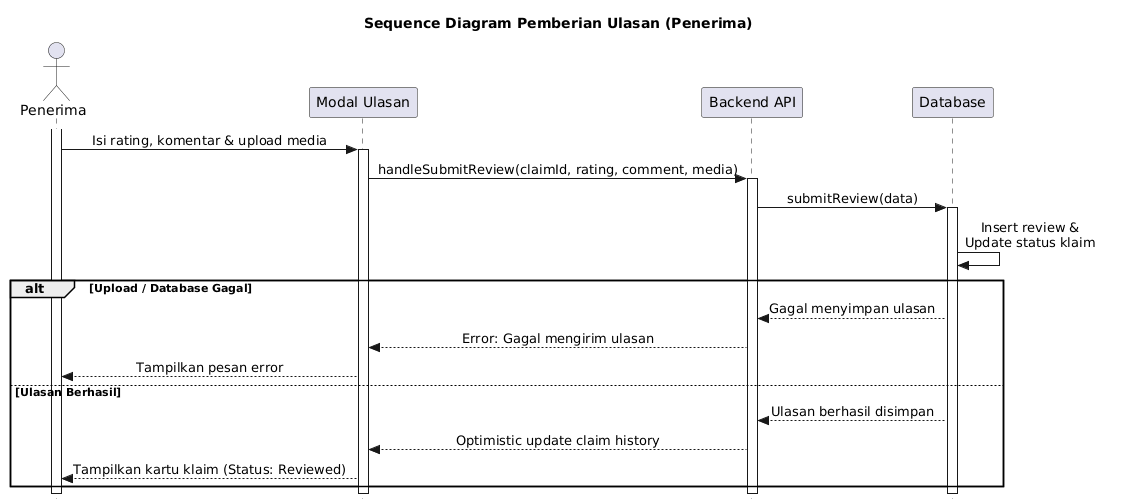
\includegraphics[width=1\textwidth]{image/bab3/sequence/Sequence Diagram Pemberian Ulasan (Penerima).png}
    \captionsetup{hypcap=false}
    \caption{\textit{Sequence Diagram} Pemberian Ulasan (Penerima)}
    \label{fig:sd-ulasan-penerima}
\end{figure}

% ------------------------------------------------------------------
\subsubsection{Alur Relawan}
% ------------------------------------------------------------------

\textbf{10. \textit{Sequence Diagram} Penerimaan Misi Pengantaran}

Relawan memilih misi dari \textit{Missions Board} dan mengklik ``Ambil Misi''. \textit{Backend} mengecek status transaksi di \textit{Database}. Jika status masih \textit{PENDING}, \textit{Backend} menetapkan ID Relawan (\texttt{volunteer\_id}) dan mengubah status menjadi \textit{IN\_PROGRESS}. Rute navigasi kemudian ditampilkan. Jika misi sudah diambil orang lain, sistem akan menolak dan memperbarui daftar misi.

\begin{figure}[H]
    \centering
    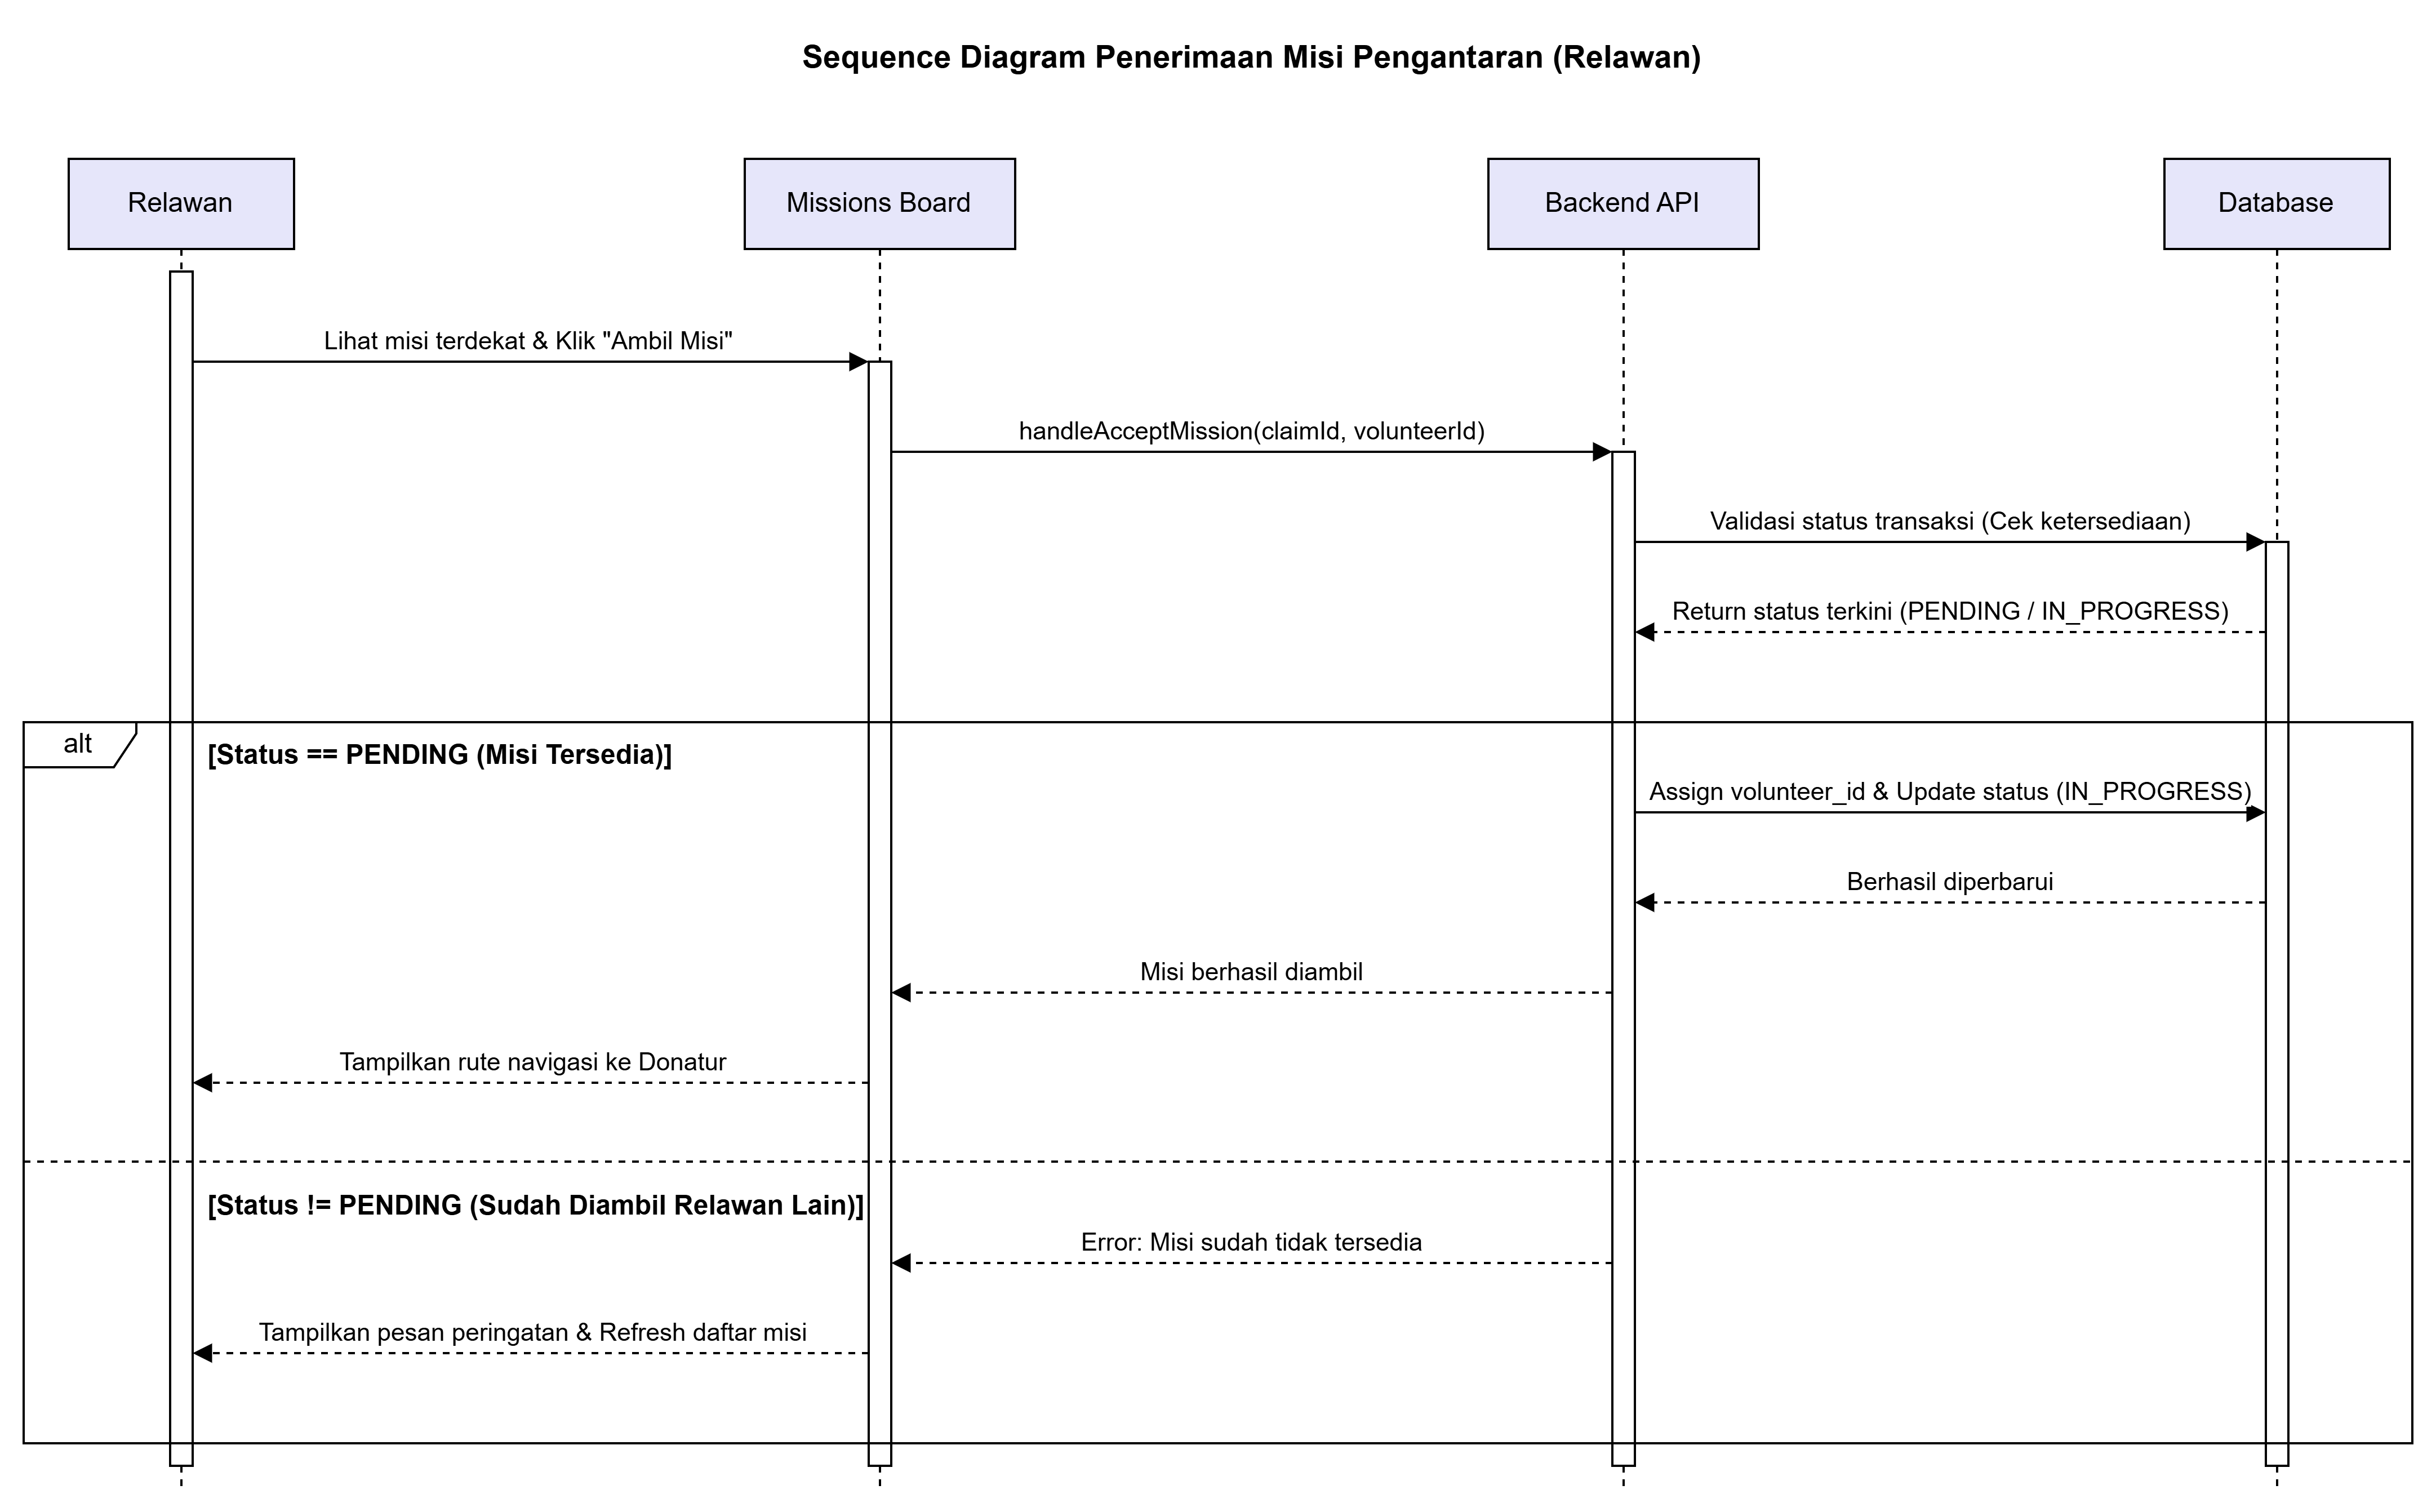
\includegraphics[width=1\textwidth]{image/bab3/sequence/Sequence Diagram Penerimaan Misi Pengantaran (Relawan).png}
    \captionsetup{hypcap=false}
    \caption{\textit{Sequence Diagram} Penerimaan Misi Pengantaran (Relawan)}
    \label{fig:sd-misi-relawan}
\end{figure}

\textbf{11. \textit{Sequence Diagram} Validasi Serah Terima (QR Code / Manual)}

Saat mengantar makanan, Relawan memindai QR Code Penerima menggunakan kamera atau mengetik \textit{Unique Code} 6-digit secara manual. \textit{Backend} memverifikasi \texttt{handleVerifyCode} dengan data di \textit{Database}. Jika cocok, status klaim diubah menjadi \textit{COMPLETED}, dan \textit{Backend} langsung memicu (\textit{trigger}) \texttt{GamificationService}.

\begin{figure}[H]
    \centering
    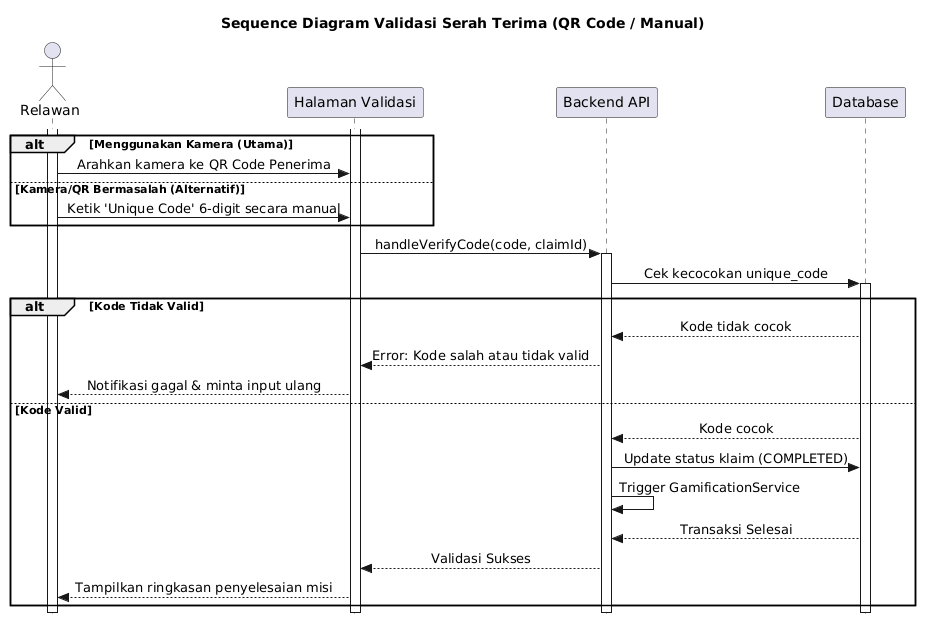
\includegraphics[width=1\textwidth]{image/bab3/sequence/Sequence Diagram Validasi Serah Terima (Relawan).png}
    \captionsetup{hypcap=false}
    \caption{\textit{Sequence Diagram} Validasi Serah Terima (Relawan)}
    \label{fig:sd-serahterima-relawan}
\end{figure}

% ------------------------------------------------------------------
\subsubsection{Alur Sistem Internal}
% ------------------------------------------------------------------

\textbf{12. \textit{Sequence Diagram} Kalkulasi Gamifikasi XP \& \textit{Badge}}

Berjalan di latar belakang tanpa interaksi langsung pengguna. Setelah validasi serah terima berhasil, \textit{Backend} meminta \texttt{calculateXP} ke \textit{Gamification Service}. Layanan mengambil poin dampak dari \textit{Database}, lalu menambahkannya ke ID Relawan. Selanjutnya, \texttt{evaluateRank} mengevaluasi total poin. Jika memenuhi syarat naik pangkat, lencana (\textit{badge}) dan \textit{rank} pengguna akan otomatis diperbarui di \textit{database}.

\begin{figure}[H]
    \centering
    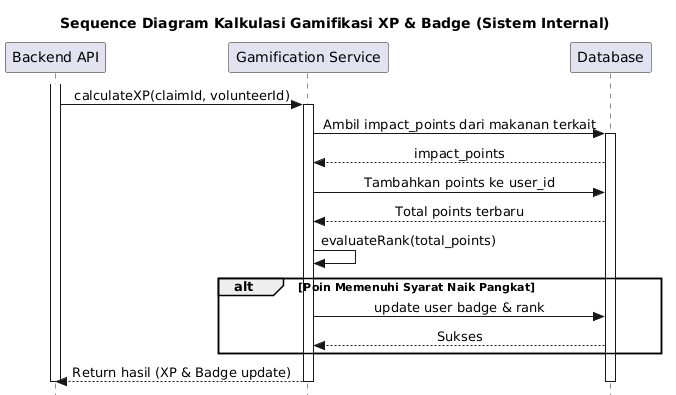
\includegraphics[width=1\textwidth]{image/bab3/sequence/Sequence Diagram Kalkulasi Gamifikasi (Sistem Internal).png}
    \captionsetup{hypcap=false}
    \caption{\textit{Sequence Diagram} Kalkulasi Gamifikasi (Sistem Internal)}
    \label{fig:sd-gamifikasi}
\end{figure}

% ------------------------------------------------------------------
\subsubsection{Alur Admin \& Super Admin}
% ------------------------------------------------------------------

\textbf{13. \textit{Sequence Diagram} Verifikasi Akun (Admin)}

Admin memilih akun pendaftar baru dan mengklik ``Verifikasi'' di \textit{User Manager}. \textit{Backend} memproses \texttt{handleVerifyUser} dan memperbarui status pengguna menjadi \textit{ACTIVE} atau \textit{REJECTED} di \textit{Database}. Setelah itu, sistem mengirimkan email notifikasi ke pendaftar, dan antarmuka Admin menampilkan status hijau.

\begin{figure}[H]
    \centering
    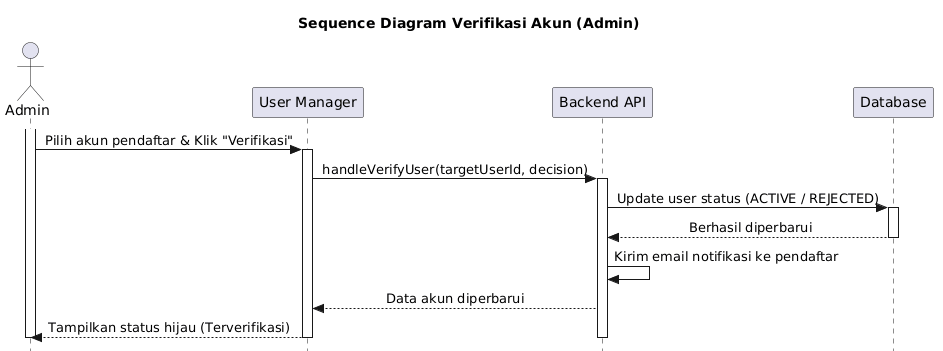
\includegraphics[width=1\textwidth]{image/bab3/sequence/Sequence Diagram Verifikasi Akun (Admin).png}
    \captionsetup{hypcap=false}
    \caption{\textit{Sequence Diagram} Verifikasi Akun (Admin Pengelola)}
    \label{fig:sd-verifikasi-admin}
\end{figure}

\textbf{14. \textit{Sequence Diagram} Moderasi Komplain (Admin)}

Admin meninjau laporan keluhan pengguna di halaman \textit{Support Request} dan memberikan keputusan. \textit{Backend} menjalankan \texttt{handleResolveReport}, lalu memperbarui tabel laporan menjadi \textit{RESOLVED} dan menyesuaikan status klaim di \textit{Database}. Kasus kemudian dihapus dari antrean aktif.

\begin{figure}[H]
    \centering
    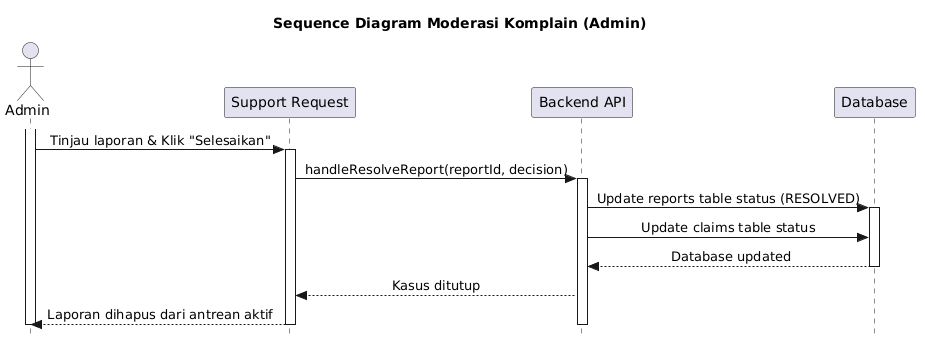
\includegraphics[width=1\textwidth]{image/bab3/sequence/Sequence Diagram Moderasi Komplain (Admin).png}
    \captionsetup{hypcap=false}
    \caption{\textit{Sequence Diagram} Moderasi Komplain (Admin Pengelola)}
    \label{fig:sd-moderasi-admin}
\end{figure}

\textbf{15. \textit{Sequence Diagram} Manajemen Status \textit{Server} (Super Admin)}

Super Admin mengakses \textit{System Config} dan menggeser tuas ``Maintenance Mode'' (ON/OFF). \textit{Backend} menerima \texttt{toggleMaintenance(boolean)} dan memperbarui kunci pengaturan di \textit{Database}. Secara sistemik, tindakan ini akan membatalkan (\textit{invalidate}) seluruh sesi aktif pengguna lain, dan memunculkan tampilan ``mode pemeliharaan'' di seluruh aplikasi.

\begin{figure}[H]
    \centering
    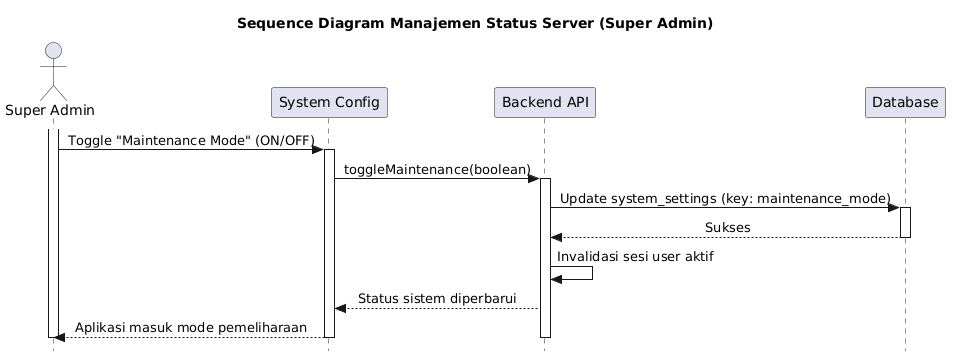
\includegraphics[width=1\textwidth]{image/bab3/sequence/Sequence Diagram Manajemen Status Server (Super Admin).png}
    \captionsetup{hypcap=false}
    \caption{\textit{Sequence Diagram} Manajemen Status \textit{Server} (Super Admin)}
    \label{fig:sd-server-superadmin}
\end{figure}

\noindent Sebagai ringkasan, seluruh \textit{sequence diagram} yang telah dipaparkan di atas dirangkum dalam tabel berikut:

\begin{longtable}{|p{0.6cm}|p{3cm}|p{4.5cm}|p{6cm}|}
    \caption{Daftar dan Spesifikasi \textit{Sequence Diagram} Food AI Rescue}
    \label{tab:ringkasan-sd} \\
    \hline
    \textbf{No} & \textbf{Peran} & \textbf{Nama \textit{Sequence Diagram}} & \textbf{Spesifikasi Pembahasan (Alur Logika)} \\
    \hline
    \endfirsthead
    \hline
    \textbf{No} & \textbf{Peran} & \textbf{Nama \textit{Sequence Diagram}} & \textbf{Spesifikasi Pembahasan (Alur Logika)} \\
    \hline
    \endhead
    \hline
    \multicolumn{4}{r}{\textit{Bersambung ke halaman berikutnya}} \\
    \endfoot
    \hline
    \endlastfoot

    1 & Global / Umum & SD Melakukan \textit{Login} & Menggambarkan alur validasi input kredensial pengguna, pencocokan data di basis data, hingga penerbitan token sesi (JWT) dan pengarahan ke \textit{dashboard} masing-masing peran. \\
    \hline

    2 & Penerima & SD Pencarian \& Klaim Makanan & Membahas proses penelusuran katalog makanan, pemilihan metode pengambilan (mandiri/kurir), pembuatan kode unik, hingga pemotongan stok pada basis data. \\
    \hline

    3 & Penerima & SD Pemberian Ulasan (\textit{Review}) & Menggambarkan alur pengiriman penilaian (bintang) dan media foto terhadap makanan/donatur setelah transaksi berstatus selesai (\textit{completed}). \\
    \hline

    4 & Penerima & SD Pelaporan Masalah (\textit{Report}) & Membahas proses pengiriman detail komplain (beserta bukti foto) yang akan mengubah status transaksi dan memicu notifikasi peringatan ke dasbor Admin. \\
    \hline

    5 & Relawan & SD Penerimaan Misi Pengantaran & Menggambarkan alur pengambilan penugasan logistik dari \textit{Missions Board}, dilengkapi dengan blok alternatif penanganan kegagalan (\textit{race condition}) jika misi ternyata sudah diklaim oleh relawan lain di waktu yang bersamaan. \\
    \hline

    6 & Relawan & SD Validasi Serah Terima (\textit{QR Code} / Manual) & Membahas komunikasi serah terima di mana relawan dapat memindai \textit{QR Code} melalui kamera, atau memasukkan 6-digit kode unik secara manual sebagai cadangan (\textit{fallback}) jika perangkat kamera bermasalah. \\
    \hline

    7 & Relawan & SD Kalkulasi Gamifikasi (Sistem Internal) & Menggambarkan proses sistem berjalan di belakang layar untuk menghitung poin dampak, menaikkan metrik \textit{Experience Point} (XP), dan memperbarui peringkat relawan secara otomatis setelah misi selesai. \\
    \hline

    8 & Donatur Individu & SD Unggah Surplus Makanan \& Verifikasi AI & Membahas alur formulir bertahap (\textit{multi-step form}) di mana donatur menginput data dan foto makanan, yang kemudian divalidasi secara langsung oleh AI (skor keamanan \& alergen) sebelum data disimpan dan dipublikasikan ke katalog. \\
    \hline

    9 & Donatur Individu & SD Konfirmasi Pesanan & Membahas proses Donatur saat menerima notifikasi klaim dari Penerima dan melakukan pembaruan status persetujuan (\textit{Approved/Ready}) pada transaksi. \\
    \hline

    10 & Donatur Individu & SD Dasbor Dampak Sosial (SROI) & Menggambarkan alur sistem saat menarik agregasi data log transaksi dan mengonversinya menjadi grafik visual reduksi emisi karbon (CO\textsubscript{2}) dan penghematan air tanah. \\
    \hline

    11 & Donatur Korporat & SD \textit{Generate} CSR \textit{Copywriter} & Membahas penarikan data transaksi aktual untuk diolah AI menjadi dua versi teks (untuk Donatur dan Penerima) dengan kustomisasi nada dan platform target, disertai fitur pengiriman \textit{request posting} ke akun Penerima. \\
    \hline

    12 & Donatur Korporat & SD Pembuatan Logo \& Rekomendasi Kemasan & Menggambarkan alur pemrosesan AI ganda, di mana sistem menghasilkan gambar logo kemasan, sekaligus menganalisis spesifikasi makanan untuk memberikan rekomendasi material kemasan (misal: anti-air) dan nama vendor di internet. \\
    \hline

    13 & Admin & SD Verifikasi \& Kelola Akun & Menggambarkan alur Admin saat menarik daftar pendaftar baru, memeriksa dokumen identitas, dan mengubah status akun menjadi aktif (terverifikasi) atau ditolak. \\
    \hline

    14 & Admin & SD Moderasi Komplain & Membahas alur resolusi sengketa, di mana Admin meninjau bukti dari Penerima/Relawan dan menetapkan keputusan status final pada log transaksi (basis data). \\
    \hline

    15 & Super Admin & SD Manajemen Status \textit{Server} & Membahas alur pengaktifan \textit{Maintenance Mode}, yang memicu pemutusan sesi (akses) publik dan mengalihkan seluruh lalu lintas pengguna ke halaman pemeliharaan. \\
    \hline

\end{longtable}

% ==============================================================================
\section{Perancangan Antarmuka Pengguna}
% ==============================================================================

Perancangan antarmuka pengguna (\textit{User Interface Design}) merupakan tahapan krusial dalam pengembangan sistem yang bertujuan untuk menjembatani interaksi antara pengguna dengan fungsionalitas di balik layar secara intuitif, efisien, dan estetis. Pada platform \textbf{Food AI Rescue}, antarmuka dirancang berbasis \textit{Progressive Web App} (PWA) menggunakan \textit{framework} React.js dengan TypeScript guna memberikan pengalaman pengguna (\textit{User Experience}/UX) yang sangat responsif, modern, dan dapat diakses dengan lancar lintas perangkat.

Secara visual, desain antarmuka aplikasi Food AI Rescue mengusung konsep premium interaktif dengan gaya tembus pandang (\textit{Glassmorphism}) yang dipadukan dengan pesona latar belakang \textit{mesh gradients}. Guna mempermudah navigasi dan interaksi, antarmuka ini juga dibekali dengan elemen visual dinamis seperti animasi alur operasional (\textit{Roadmap}) dan \textit{cursor follower} khusus yang dirancang untuk memandu pengguna baru dalam menjelajahi ekosistem aplikasi.

Selain itu, tata letak setiap layar dirancang secara eksklusif mengikuti arsitektur hak akses (\textit{Role-Based Access Control}), sehingga masing-masing pengguna (Donatur Individu, Donatur Korporat, Penerima, Relawan, Admin, dan Super Admin) mendapatkan menu dan dasbor yang relevan dengan tugas mereka, mulai dari panel verifikasi keamanan pangan AI, pelacakan rute navigasi \textit{booking}, \textit{leaderboard} gamifikasi relawan, hingga visualisasi Dasbor Dampak Sosial (SROI).

\subsection{Antarmuka Pemasaran Publik dan Autentikasi}

% Tambahkan gambar dan penjelasan antarmuka halaman publik dan login di sini

\subsection{Antarmuka Dasbor Donatur (Individu dan Korporat)}

% Tambahkan gambar dan penjelasan antarmuka dasbor donatur di sini

\subsection{Antarmuka Dasbor Penerima Donasi}

% Tambahkan gambar dan penjelasan antarmuka dasbor penerima di sini

\subsection{Antarmuka Dasbor Relawan}

% Tambahkan gambar dan penjelasan antarmuka dasbor relawan di sini

\subsection{Antarmuka Dasbor Admin dan Super Admin}

% Tambahkan gambar dan penjelasan antarmuka dasbor admin dan super admin di sini

% ==============================================================================
\section{Kebutuhan Perangkat Keras dan Perangkat Lunak}
% ==============================================================================

Guna menunjang keberhasilan rancang bangun platform \textit{Food AI Rescue}---baik pada fase rekayasa lokal maupun penerapan di tingkat produksi (\textit{deployment})---diperlukan spesifikasi infrastruktur teknologi yang terukur dan andal. Subbab ini merincikan daftar kebutuhan spesifikasi minimum perangkat keras (\textit{hardware}) dan perangkat lunak (\textit{software}) yang berfungsi sebagai lingkungan operasional (\textit{environment}) bagi sistem basis data, peladen \textit{backend}, integrasi API \textit{Machine Learning}, hingga perangkat akses akhir yang digunakan oleh pengguna di lapangan.

\subsection{Pengembangan Sistem}
\label{subsec:kebutuhan-pengembangan}

Kebutuhan perangkat keras (\textit{hardware}) yang digunakan oleh penulis dalam proses pembuatan dan pengembangan platform \textit{Food AI Rescue} adalah sebagai berikut:

\begin{longtable}{|p{0.5cm}|p{2.8cm}|p{5.5cm}|p{4.8cm}|}
    \caption{Kebutuhan Perangkat Keras (\textit{Hardware}) Pengembangan}
    \label{tab:hardware-dev} \\
    \hline
    \textbf{No} & \textbf{Perangkat} & \textbf{Fungsi} & \textbf{Spesifikasi} \\
    \hline
    \endfirsthead
    \hline
    \textbf{No} & \textbf{Perangkat} & \textbf{Fungsi} & \textbf{Spesifikasi} \\
    \hline
    \endhead
    \hline
    \multicolumn{4}{r}{\textit{Bersambung ke halaman berikutnya}} \\
    \endfoot
    \hline
    \endlastfoot
    1 & Laptop & Digunakan sebagai \textit{workstation} utama untuk mengembangkan dan menjalankan program atau aplikasi. & Lenovo IdeaPad 3 14IAU7 \\
    \hline
    2 & Prosesor & Berfungsi memproses instruksi komputasi dan menjalankan arsitektur aplikasi \textit{client-server}. & 12th Gen Intel(R) Core(TM) i3-1215U (1.20 GHz) \\
    \hline
    3 & RAM & Memori sementara yang mendukung kinerja sistem saat mengompilasi kode dan mengolah data secara lokal. & 8 GB DDR4 \\
    \hline
    4 & Penyimpanan & Menyimpan sistem operasi, data \textit{database}, dan \textit{source code} proyek agar dapat diakses dengan cepat. & SSD 512 GB \\
    \hline
    5 & Monitor & Menampilkan antarmuka kode serta pratinjau \textit{output} dari \textit{Progressive Web App} (PWA) yang dibangun. & 14 inch, resolusi 1920$\times$1080 (\textit{Full HD}) \\
    \hline
    6 & \textit{Keyboard} & Alat \textit{input} untuk mengetik skrip kode pemrograman dan memberikan perintah operasional ke komputer. & -- \\
    \hline
    7 & Internet & Sarana krusial untuk mengakses dokumentasi, mengunduh \textit{library} NPM, serta mengakses \textit{Google Gemini API}. & -- \\
    \hline
\end{longtable}

Perangkat lunak (\textit{software}) meliputi sistem operasi, bahasa pemrograman, \textit{framework}, dan alat desain yang digunakan oleh penulis dalam merancang hingga membangun aplikasi \textit{Food AI Rescue} di lingkungan lokal. Rinciannya adalah sebagai berikut:

\begin{longtable}{|p{0.5cm}|p{3.5cm}|p{5cm}|p{4.5cm}|}
    \caption{Kebutuhan Perangkat Lunak (\textit{Software}) Pengembangan}
    \label{tab:software-dev} \\
    \hline
    \textbf{No} & \textbf{Perangkat} & \textbf{Fungsi} & \textbf{Spesifikasi} \\
    \hline
    \endfirsthead
    \hline
    \textbf{No} & \textbf{Perangkat} & \textbf{Fungsi} & \textbf{Spesifikasi} \\
    \hline
    \endhead
    \hline
    \multicolumn{4}{r}{\textit{Bersambung ke halaman berikutnya}} \\
    \endfoot
    \hline
    \endlastfoot
    1 & Sistem Operasi & Menyediakan platform dasar untuk menjalankan dan mengelola seluruh aplikasi pengembangan. & Windows 11 Home Single Language \\
    \hline
    2 & Lingkungan \textit{Backend} (Node.js \& Express.js) & Lingkungan eksekusi utama dan \textit{framework} API untuk memproses logika bisnis sistem di sisi server lokal. & Node.js / Express (v5.x) \\
    \hline
    3 & Lingkungan \textit{Frontend} (React.ts \& Vite) & \textit{Framework} berbasis komponen dan \textit{build-tool} untuk merancang antarmuka pengguna (UI) yang reaktif. & React.js (v19) dengan TypeScript \\
    \hline
    4 & XAMPP / Laragon & Perangkat lunak \textit{web server} lokal yang menyediakan layanan modul pangkalan data. & Modul MySQL \\
    \hline
    5 & MySQL & Sistem manajemen basis data (RDBMS) utama untuk menyimpan dan mengelola rekam jejak data aplikasi. & MySQL (MariaDB) versi 10.4.32 \\
    \hline
    6 & VSCode & \textit{Text editor} utama yang digunakan untuk penulisan \textit{source code} pengembangan aplikasi. & Version 1.102.2 \\
    \hline
    7 & Google Chrome & Peramban utama untuk menguji \textit{debugging} dan menjalankan aplikasi web secara lokal (\textit{localhost}). & Version 138.0.7204.168 \\
    \hline
    8 & Figma & Alat desain antarmuka pengguna untuk membuat prototipe, \textit{wireframe}, dan merancang gaya \textit{Glassmorphism}. & Versi berbasis web \\
    \hline
    9 & Draw.io \& PlantUML & Alat bantu visualisasi untuk merancang berbagai pemodelan \textit{Unified Modeling Language} (UML) dan BPMN. & Versi berbasis web \\
    \hline
    10 & Google Gemini Vision API & Layanan Kecerdasan Buatan (AI) pihak ketiga untuk fitur verifikasi kelayakan makanan dan konten generatif. & API / \textit{Cloud Service} \\
    \hline
\end{longtable}

\subsection{Implementasi Sistem}
\label{subsec:kebutuhan-implementasi}

Agar platform \textit{Food AI Rescue} dapat dieksekusi dan dikembangkan secara optimal pada perangkat komputasi lain, dibutuhkan spesifikasi minimal untuk perangkat keras (\textit{hardware}) maupun perangkat lunak (\textit{software}) sebagai berikut:

\begin{longtable}{|p{0.5cm}|p{2.8cm}|p{5.5cm}|p{4.8cm}|}
    \caption{Kebutuhan Perangkat Keras dan Perangkat Lunak (Minimal) dalam Pengerjaan TA}
    \label{tab:hardware-impl} \\
    \hline
    \textbf{No} & \textbf{Perangkat} & \textbf{Fungsi} & \textbf{Spesifikasi (Minimal)} \\
    \hline
    \endfirsthead
    \hline
    \textbf{No} & \textbf{Perangkat} & \textbf{Fungsi} & \textbf{Spesifikasi (Minimal)} \\
    \hline
    \endhead
    \hline
    \multicolumn{4}{r}{\textit{Bersambung ke halaman berikutnya}} \\
    \endfoot
    \hline
    \endlastfoot
    1 & Laptop/PC & Digunakan sebagai \textit{workstation} utama untuk merancang, memprogram, dan menjalankan arsitektur aplikasi \textit{client-server}. & Prosesor Intel Core i3 (atau setara) ke atas \\
    \hline
    2 & RAM & Menjaga stabilitas kinerja sistem komputasi saat mengeksekusi server lokal dan memproses kompilasi kode. & 8 GB \\
    \hline
    3 & Sistem Operasi & Menyediakan lingkungan dasar yang mendukung jalannya \textit{tools} pengembangan aplikasi berbasis web. & Windows 10/11, macOS, atau Linux \\
    \hline
    4 & VSCode & Penyunting kode (\textit{text editor}) utama untuk menulis, mengelola, dan melakukan \textit{debugging} pada \textit{source code frontend} maupun \textit{backend}. & Versi 1.59.x atau yang lebih baru \\
    \hline
    5 & Node.js & Lingkungan eksekusi utama untuk menjalankan kerangka kerja server \textit{backend} (Express.js), \textit{frontend} (React), dan integrasi API. & Versi 18.x LTS atau yang lebih tinggi \\
    \hline
\end{longtable}
